\documentclass[11pt,a4paper]{article}

%, Page Geometry & Layout ,
\usepackage[margin=1in]{geometry}
\usepackage[utf8]{inputenc}
\usepackage[T1]{fontenc}
\usepackage{lmodern}

%, Core Math & Symbols ,
\usepackage{amsmath,amssymb,amsfonts,amsthm}

%, Graphics, Tables & Formatting ,
\usepackage{graphicx}
\usepackage{booktabs}
\usepackage{microtype}
\usepackage{setspace}
\onehalfspacing

%, Tables ,
\usepackage{array}
\usepackage{multirow}
\usepackage{tabularx}
\renewcommand{\arraystretch}{1.15}
\setlength{\tabcolsep}{6pt}
\newcolumntype{R}{>{\raggedleft\arraybackslash}X}
\newcolumntype{L}{>{\raggedright\arraybackslash}X}
\newcommand{\tabfont}{\footnotesize}
\newcommand{\thead}[1]{\footnotesize\textbf{#1}}

%, Captions ,
\usepackage{caption}
\captionsetup{font=small, labelfont=bf}

%, Lists ,
\usepackage{enumitem}
\setlist[itemize]{leftmargin=1.5em,itemsep=2pt,topsep=4pt,parsep=0pt}
\setlist[enumerate]{leftmargin=1.8em,itemsep=2pt,topsep=4pt,parsep=0pt}

%, Colors ,
\usepackage[table,dvipsnames]{xcolor}
\definecolor{arblue}{HTML}{2A78D6}
\definecolor{dgorange}{HTML}{EB6834}
\definecolor{llaqua}{HTML}{1BAF7A}
\definecolor{linkc}{HTML}{1B3A5C}

%, Hyperlinks & Metadata ,
\usepackage[
    colorlinks=true,
    linkcolor=linkc,
    citecolor=linkc,
    urlcolor=linkc,
    pdfauthor={Aleksandr Kaigorodov},
    pdftitle={Diffusion LLMs as Fast Models for Specific Tasks},
    pdfsubject={Block-structured decoding cost analysis},
    pdfkeywords={diffusion LLM, block decoding, latency, structured output}
]{hyperref}

%, Model shorthands ,
% NB: \ARthree renders AR-30B (the name is an AR-3B-era leftover).
\newcommand{\ARthree}{\textsc{ar-30b}}
\newcommand{\DG}{\textsc{dg}}
\newcommand{\LLaDA}{\textsc{llada-8b}}

%, Macros (numbers from results/) ,
% =============================================================================
%  macros.tex — every number the paper cites, in one place.
%
%  Rule: every measurement is a macro here, and the comment on its line names
%  the artifact it was read from. Section files may hardcode derived ratios
%  (e.g., 2.5×) and structural constants (e.g., 12 fields, $K{=}8$) for
%  readability, but raw measurements (latencies, F1 scores, energy) must be
%  macros. paper/verify_numbers.py checks provenance blocks and decimal-place
%  policy; the figure builder (paper/figures/make_figures.py) prints what it
%  plotted so the two can be diffed.
% =============================================================================

% --- Pinned stack -------------------------------------------------- (#57) --
\newcommand{\gpuModel}{NVIDIA A100 80GB PCIe}
% prompt_token_count in every DG cell (issue68_dg_L*.json, 42 files). The AR
% cells run shorter prompts (992); 1,077 is the DG figure the crossover is
% calibrated at. Was 1,047 -- a stale constant from docs/edr/005, no artifact.
\newcommand{\refPrompt}{1{,}077}

% --- Quality, 9-field vs 12-field ----- results/issue43_nine_field_f1.json --
\newcommand{\arThreeBFnine}{0.852}     % dense AR-3B (Qwen2.5-3B), L=256, 9-field, re-scored (#43)
\newcommand{\qualityGap}{0.000}        % |9-field difference|
\newcommand{\twelveGap}{0.041}         % 12-field difference, AR-favoured

% --- Cost laws ------------- results/anchors/*.json, results/issue68_*.json --
% AR-30B (arBase/arSlope/crossoverL): results/issue111_qwen3_serial_sweep.json
%   cost_law.{intercept_ms,slope_ms_per_token,crossover_L_star}. UNVERIFIED --
%   inherited from the gold-leaked harness (issue #112); pending re-measurement
%   on the pinned stack. verify_numbers.py errors until provenance is present.
\newcommand{\arBase}{34.6}        % ms, AR-30B MoE serial intercept (Qwen3-30B-A3B)
\newcommand{\arSlope}{7.2}       % ms/token, AR-30B MoE serial decode slope
\newcommand{\dgBase}{378.8}       % ms, DG base at K=8
\newcommand{\dgStep}{119.5}       % ms, median of the 7 measured canvas steps
\newcommand{\dgStepLo}{113.1}     % ms, smallest measured step (1280->1536)
\newcommand{\dgStepHi}{122.6}     % ms, largest measured step (256->512)
\newcommand{\canvasLength}{256}   % tokens per canvas

% Anchors, five repeats each -------- results/anchors/anchor_remeasure.json --
% Per-event dispersion: n=2000 (issue #120, was n=300 where p99.9==max)
% results/anchors/dg_L256_r1_preds.jsonl, ar3b_L256_n2000_preds.jsonl
\newcommand{\arEventCV}{0.1}     % % CV over 2000 per-event latencies (AR-3B dense)
\newcommand{\dgEventCV}{16.9}
\newcommand{\arMaxMed}{1.03}      % max / median per-event latency (AR-3B dense)
\newcommand{\dgMaxMed}{3.07}

% --- Crossovers ------- derived from arBase/arSlope/dgBase above --------------
% NB: models/decision/procedure.py still records the AR-3B-era values
% (l_cross_tokens=65, lambda_cross_ev_s=1.8); it is NOT the source of these.
\newcommand{\crossoverL}{48}       % tokens: (dgBase - arBase) / arSlope, serial mode
\newcommand{\crossoverLambda}{2.6} % ev/s: 1000 / dgBase (unchanged — DG base same)

% --- Input length, the second variable ------ results/issue44_*_sweep.json --
\newcommand{\inputSlopeRatio}{2.6} % dgInputSlope / arInputSlope (0.1/0.038)

% --- Base decomposition ------------------- results/issue44_dg_ksweep_K*.json --
\newcommand{\kfitBase}{296.1}      % ms, K-independent term (NOT interpretable as a floor; see #70)
\newcommand{\kfitSlope}{2.6}      % ms per denoising step
\newcommand{\kfitRsq}{0.49}
% Superseded: the fitted intercept (296.1) is not a measured floor. R^2=0.49
% and the curve saturates above K=16, so the linear term is a poor description.
% The 93.5%/6.5% split it produced over-attributes to the floor by ~5x.
% Replaced by two measurement-based bounds (issue #70):
% Floor share <=53% (from T(2)=201.7ms), denoising share >=32% (from canvas step 119.5ms).
% Values are hardcoded in Appendix 10 (appendix_decomp.tex).

% --- Batching ------------------- results/issue42_batching.json, appD, dInfer --
% NB: #42 was run on the dense AR-3B (Qwen2.5-3B-Instruct), NOT the AR-30B MoE.
% The AR-30B MoE multiplier is 24.7x (results/issue111_qwen3_batch_sweep.json).
\newcommand{\cacheOnMult}{42.8}    % dense AR-3B, prefix caching on   (#42)
\newcommand{\cacheOffMult}{26.8}   % dense AR-3B, prefix caching off  (#42)
\newcommand{\dgBatchVllmHi}{1.7}   % DG under vLLM, L=128 (lower bound)

% --- Energy ------------------------------------- three separate artifacts ---
% Values hardcoded in sec 03 (03_deployment.tex). Each comes from its own file:
%   DG      4.2 J, idle 52.6W  -- results/issue_energy_measurement.json
%   AR-30B 118.7 J, idle 49.7W  -- results/issue111_ar30b_energy.json (serial, 928 ms/event;
%                                 re-measured issue #112, was 10.1 J batch-served)
%   AR-1.5B 5.1 J, idle 58.6W  -- results/issue_evidence_ar1b_energy.json
% Ratios 118.7/4.2 = 28.3 (serial/serial) and 5.1/4.2 = 1.2. The AR-30B
% energy run is now serial (928 ms/event), matching DG's serial regime.

% --- Deployment pair ------ results/issue_evidence_ar1b_*.json, issue68_*.json --
\newcommand{\dgWeights}{52.0}          % GB, bf16

% --- Defect magnitudes ------------------------------ CHECKLIST.md, #65 -----
\newcommand{\defectOneFBefore}{0.779}
\newcommand{\defectOneFAfter}{0.844}
\newcommand{\defectTwoBefore}{1841.6}
\newcommand{\defectTwoAfter}{413.3}
\newcommand{\defectTwoRatio}{4.5}
\newcommand{\defectThreeBefore}{0.599}
\newcommand{\defectThreeAfter}{0.826}
\newcommand{\defectFourBefore}{0}
\newcommand{\defectFourAfter}{100}
\newcommand{\rambleRate}{96}      % % of AR outputs with >1 JSON object at L=512

% --- Truncation regime -------------------------- results/issue43/*.json -----
\newcommand{\arFOneTwentyEight}{0.669}   % AR-3B (dense) 9-field F1 at L=128
\newcommand{\dgFOneTwentyEight}{0.311}   % DG    9-field F1 at L=128
\newcommand{\arValidTwentyEight}{66.7}   % AR-3B (dense) schema-valid % at L=128
\newcommand{\dgValidTwentyEight}{1.0}    % DG schema-valid % at L=128

% --- Generalisation to HDFS ---------------------- results/issue67_*.json ----
\newcommand{\hdfsStep}{120.5}     % ms, DG canvas step on HDFS
\newcommand{\bglStep}{118.5}      % ms, DG canvas step on BGL (same cells)

% --- Canvas tuning -------------------------- results/issue66_canvas_*.json --
\newcommand{\canvasOneTwentyEightBase}{368.5}  % ms at canvas=128
\newcommand{\canvasOneTwentyEightFone}{0.864} % 9-field F1 at canvas=128

% --- K as a runtime quality knob --------- results/issue44_dg_ksweep_K*.json --
\newcommand{\kFourPninetynine}{394.3} % ms
\newcommand{\kFourFone}{0.790}
\newcommand{\kEightFone}{0.853}



\graphicspath{{../}{../figures/}}

\title{\textbf{Diffusion LLMs as Fast Models for Specific Tasks:\\
The Cost Shape of Block-Structured Decoding}}

\author{
  \textbf{Aleksandr Kaigorodov, Yandex}
}

\date{}

\begin{document}

\maketitle

\begin{abstract}
Autoregressive decoding has a cost that grows linearly with
output length. Block-diffusion decoding has a stepwise cost:
flat within a fixed block, stepping only at block boundaries. We
compare both paradigms on a controlled benchmark for structured log
extraction. We use a matched pair of MoE models on a single vLLM
stack. The two costs cross at a short output length. Beyond this
crossover, block-diffusion is $2.5\times$ faster at the model's
natural output length, where the autoregressive model emits
end-of-sequence. The advantage narrows toward parity for longer
outputs. The autoregressive model is preferred under high-throughput
batching, where it achieves better utilization and lower tail latency.
Block-diffusion is preferred where requests arrive serially:
investigation chains, autonomous driving, algorithmic trading. Under
a tightening deadline, block-diffusion degrades output quality
rather than truncating. We state the conditions that define when
block-diffusion decoding is the right choice.
\end{abstract}

\begin{figure}[ht!]
\centering
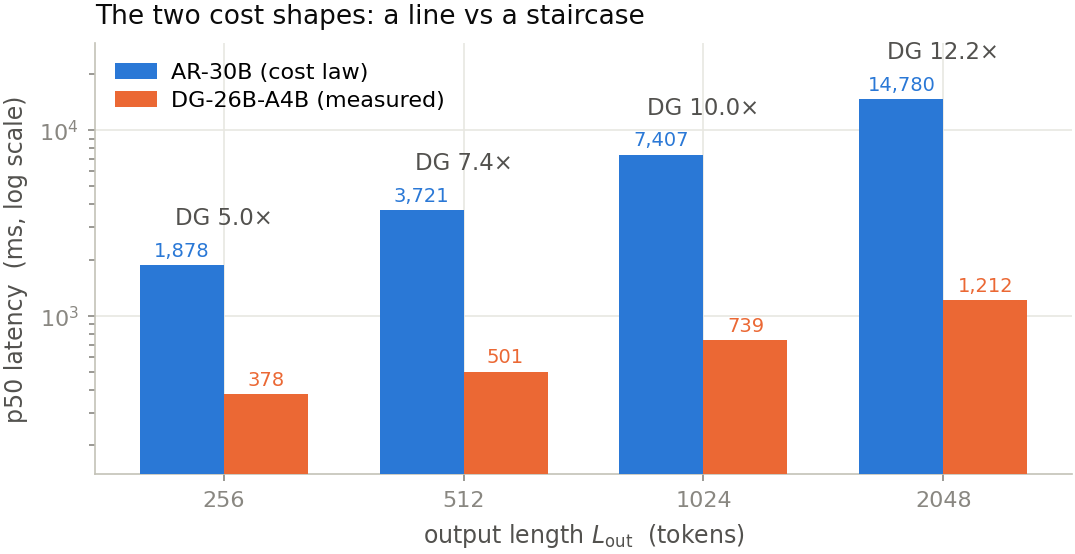
\includegraphics[width=\linewidth]{figures/fig1_cost_shapes.png}
\caption{The two cost shapes, priced at four output lengths (log scale).
Autoregressive cost grows linearly with no floor; block-diffusion cost
is a bounded staircase, flat inside each 256-token canvas and stepping
by $\sim$120\,ms at each boundary. The gap widens with output length.
Block diffusion measured (BGL, $n{=}200$, $K{=}8$); autoregressive from
the fitted serial cost law.}
\label{fig:shapes}
\end{figure}

\section{Introduction}
\label{sec:intro}

Autoregressive language models generate text one token at a time;
each token requires a forward pass over the growing key-value (KV)
cache. This is the decoding equivalent of a metered taxi: the fare
climbs with every token. Block-diffusion models generate an entire
block of tokens in
parallel through iterative denoising, then step to the next block.
The cost is a bounded staircase: flat within a fixed-size block,
stepping at each boundary. We call this second class \emph{block-diffusion} because
the block structure, not the diffusion process, is what
determines its cost shape. Figure~\ref{fig:schematic} illustrates
the two decoding patterns.

We ran both architectures on vLLM~\cite{vllm2023} on a single
\gpuModel{} to remove the serving-path asymmetry that dominates naive
comparisons. Both models were re-measured on the same pinned stack
(vLLM 0.25.1); the AR-30B was initially run on an older engine, a
defect caught and corrected (Appendix~\ref{app:defects}). The task is structured log
extraction: each raw log line describes a hardware or software event,
and the model must emit a JSON record with twelve fields spanning
structural, semantic, anomaly, and action categories. Structural
fields require span-copying from the input, semantic fields require
inference, and anomaly fields require binary classification.

\paragraph{Data.}

The corpus is BGL from LOGHUB~\cite{loghub}, 4{,}747{,}963 lines of
console log from the BlueGene/L supercomputer at Lawrence Livermore
National Laboratory, whose first column tags each line as an alert or
non-alert. We sample 600{,}000 lines uniformly (reservoir sampling,
seed 42) and split them temporally: the most recent 200{,}000 form the
test split and the remaining 400{,}000 the train split. The test split
carries 41{,}005 alert-tagged lines, an anomaly rate of $20.5\%$, so
the two anomaly fields are not degenerate. Gold records are produced
by parsing each line with Drain~\cite{drain} and carrying the native
alert tags through as \texttt{is\_anomaly} and \texttt{anomaly\_score}.

\paragraph{An example.}
The raw line
\begin{quote}\small\ttfamily
- 1118772771 R21-M0-NF-C:J11-U11 RAS KERNEL FATAL floating point instr.
\end{quote}
yields the gold record \texttt{\{"severity":"FATAL","is\_anomaly":true,\ldots\}}.
The first six fields are span-copied from the input (structural);
\texttt{is\_anomaly} and \texttt{anomaly\_score} carry the native alert
tag (anomaly); the three excluded semantic fields are parser
placeholders, not ground truth.

Quality is macro-averaged token-level F1 over 9 of the 12 fields. The
three excluded, \texttt{event\_type}, \texttt{affected\_entity} and
\texttt{remediation\_hint}, are the semantic fields whose gold
labels are parser placeholders instead of ground truth. Scoring them
measures agreement with Drain, not extraction quality. This was one of
the nine corrections priced in Appendix~\ref{app:defects}.
A record is \emph{schema-valid} if it parses as JSON and carries all
twelve keys; schema completeness is the fraction of keys present, which
separates a truncated record from a complete one. Latencies are
reported as percentiles over per-event wall time. p50 is the median;
p99 and p99.9 are the tail. Every evaluation cell draws $n = 300$ events
from the test split unless stated otherwise. For the generalisation check in \S\ref{sec:laws} we
additionally use the LOGHUB HDFS sample (2{,}000 lines, evaluation
only).

Both are Mixture-of-Experts models:
\begin{itemize}[nosep]
\item \DG\ (DiffusionGemma-26B-A4B~\cite{diffusiongemma}, 4.0\,B active
  of 26\,B total, 52\,GB), the block-diffusion (DG) model. Top-8 of 128
  experts.
\item \ARthree\ (Qwen3-30B-A3B~\cite{qwen25}, 3.0\,B active of 30\,B
  total, 60\,GB), the autoregressive (AR) model. Matched to DG on
  architecture class and active parameters.
\end{itemize}
The cost shapes we derive are properties of the \emph{decoding
paradigm}, not of model scale. A larger AR model would have a steeper
slope but the same linear shape; a larger block-diffusion model would have a
higher floor but the same staircase. Decoding parameters are matched
across models: greedy sampling (\texttt{temperature}${=}0$,
\texttt{top\_p}${=}1.0$, \texttt{repetition\_penalty}${=}1.0$) on
both; DG runs at $K{=}8$ denoising steps with canvas $C{=}256$. The
full parameter set is recorded in each result artifact's
\texttt{provenance} block.

\paragraph{Measurement corrections.}

Eight measurement defects were found by re-reading our own committed
artifacts: a checkpoint default that suppressed span-copying, a parser
that took the most-drifted JSON object, a metric that counted falsy
values as missing keys. Five of the eight biased against AR.
The reported advantage survives all nine corrections --- the eight
defects plus a switch to an architecture-matched AR baseline. The
corrections are priced in Appendix~\ref{app:defects}; they are the
methodological basis of every number that follows.

Our contributions are as follows:
\begin{itemize}[leftmargin=1.5em]
\item \textbf{How do the two architectures differ in latency cost?}
We derive two cost laws from measurement: AR latency is a line in output
length with no floor; block-diffusion latency is a staircase, flat inside
a fixed-size block and stepping at each boundary. The shapes cross at
$L^{*} = \crossoverL$ output tokens (\S\ref{sec:laws}).

\item \textbf{Where is block-diffusion faster?}
Above $L^{*}$, DG is faster, two and a half times at natural output,
narrowing to just over parity at a thousand tokens. In cost terms, that is the difference
between \$0.0012 and \$0.0005 per event on an A100, a gap that
compounds to hundreds of dollars at million-event scale
(\S\ref{sec:wins}).

\item \textbf{What limits DG's advantage operationally?}
AR batches far better and has a tighter tail. However, in the
batch-1 regime (serial chains, autonomous driving, trading), batching is
unavailable and the staircase shape dominates
(\S\ref{sec:limits}).

\item \textbf{When is block-diffusion the right choice?}
When output is long, batch-1 is required, and schema completeness
matters. We state five conditions and ground them in concrete
workloads (\S\ref{sec:survives}).
\end{itemize}

Table~\ref{tab:summary} states the whole comparison in one place: the
two models are matched on architecture class and footprint, and every
line after it either explains one of these rows or bounds it.

\begin{table}[h]
\centering
\caption{The paper in one table. DG's latency
advantage is real; deployment factors limit it operationally.
Max/median is the largest per-event latency over its median, across
300 events at $L{=}\canvasLength$; the AR entry for that row is the
dense AR-3B baseline, measured per-event for quality, while
every other AR entry is the AR-30B MoE.}
\label{tab:summary}
\begin{tabularx}{\linewidth}{@{}L r r@{}}
\toprule
& \thead{\ARthree\,(MoE)} & \thead{\DG-26B-A4B\,(MoE)} \\
\midrule
\tabfont Active parameters                            & 3.0\,B & 4.0\,B \\
\tabfont Total parameters                             & 30\,B & 26\,B \\
\tabfont Weights (bf16)                                & 60\,GB & 52\,GB \\
\tabfont Marginal cost (ms/token, serial) & \arSlope & 0.47 (amortised over a canvas) \\
\tabfont Batch-1 $\to$ peak throughput multiplier     & 25$\times$ & $\leq$1.7$\times$ \\
\tabfont Tail latency (max/median)                    & 1.03$\times$ & 3.21$\times$ \\
\bottomrule
\end{tabularx}
\end{table}

\begin{table}[h]
\centering
\caption{The two decoding paradigms as cost laws. AR pays per token;
DG pays per canvas. Within a canvas, DG tokens are free.}
\label{fig:schematic}
\renewcommand{\arraystretch}{1.4}
\begin{tabularx}{\linewidth}{@{}L L L@{}}
\toprule
& \thead{Autoregressive} & \thead{Block-diffusion} \\
\midrule
\tabfont Decoding & $t_1 \to t_2 \to \cdots \to t_L$ & $\{t_1, \ldots, t_C\}_K \to \{t_{C+1}, \ldots\}_K$ \\
\tabfont Cost law & $T = a + b \cdot L$ & $T = a + b \cdot \lceil L/C \rceil$ \\
\tabfont Per-token cost & $b$ (one forward pass) & $0$ (denoised in parallel) \\
\tabfont Per-canvas cost & --- & $b$ ($K$ denoising passes) \\
\tabfont Shape & linear & staircase \\
\bottomrule
\end{tabularx}
\end{table}

\section{Background: autoregressive vs block-diffusion decoding}
\label{sec:laws}

\subsection{How the two architectures decode}

\paragraph{Autoregressive (AR).}
The model generates output one token at a time. Each token requires a
forward pass over the full model and the growing KV cache. The model
cannot begin token $t_{i+1}$ until it has finished $t_i$. The cost is
strictly sequential: one forward pass per token, with no parallelism
within the sequence.

\paragraph{Block-diffusion (DG).}
The model generates an entire canvas of $C$ tokens in parallel
through $K$ iterative denoising passes. On each pass, the model
refines all $C$ token positions simultaneously: it starts from noise,
predicts cleaner tokens at every position, and repeats. After $K$
passes the canvas is fully decoded and the model steps to the next
canvas. Within a canvas, all $C$ positions are denoised in parallel,
so the marginal cost of additional tokens is zero up to $C$. The cost
jumps only at the canvas boundary, when a fresh block of $K$ denoising
passes begins.

Table~\ref{fig:schematic} contrasts the two patterns. AR cost grows
linearly with output length; DG cost is a bounded staircase.

\subsection{The cost laws}

Both laws share the structure $T = a + b \cdot f(L)$, where $a$ is the
fixed cost, $b$ is the marginal cost, and $f$ is linear for AR but a
staircase for DG. The measured forms are:
\begin{align}
\label{eq:ar}
T_{\textsc{ar}}(L_{\mathrm{out}}) &= \arBase + \arSlope \cdot L_{\mathrm{out}} && \text{(ms, linear)} \\
\label{eq:dg}
T_{\textsc{dg}}(L_{\mathrm{out}}) &= \dgBase + \dgStep \cdot \Bigl(\bigl\lceil \tfrac{L_{\mathrm{out}}}{\canvasLength}\bigr\rceil - 1\Bigr) && \text{(ms, staircase)}
\end{align}

For AR, the intercept is the prompt prefill cost, amortised by prefix
caching; the slope is one KV-cache forward pass per token. For DG, the
intercept is the first-canvas cost: the prompt is re-attended $K$
times, once per denoising step. The slope is the cost of one additional
canvas. The operating point $K{=}8$ was selected as the latency/quality
knee: quality is approximately flat above $K{=}8$ while latency
saturates above $K{=}16$.

AR is a metered taxi: the fare climbs with every token; DG is a
subway with a flat fare per station. The shapes cross where the two costs
are equal. Solving for $L_{\mathrm{out}}$:
\begin{equation}
\label{eq:lcross}
L^{*} = \frac{a_{\textsc{dg}} - a_{\textsc{ar}}}{b_{\textsc{ar}}}
= \frac{\dgBase - \arBase}{\arSlope} = \crossoverL \text{ tokens},
\qquad
\lambda^{*} = \frac{1000}{a_{\textsc{dg}}} = \frac{1000}{\dgBase} = \crossoverLambda \text{ events/s}
\end{equation}
where $L^{*}$ is the crossover output length and $\lambda^{*}$ is the
maximum serial event rate before a queue forms. Below $L^{*}$, AR is
cheaper. Above it, DG is permanently cheaper, but not smoothly. The DG
advantage grows within each canvas as AR cost increases. It resets at
each canvas boundary, where DG incurs the cost of the next block, then
grows again. The crossover $L^{*}$ shifts with input length. DG's
prompt is re-attended $K$ times, making its input slope
$\sim$2.6$\times$ steeper than the dense AR-3B's (0.123 against
0.047\,ms per prompt token). Longer prompts raise the base and push
$L^{*}$ upward (Appendix~\ref{app:input_canvas}).
Figure~\ref{fig:shapes} (page~\pageref{fig:shapes})
plots the two shapes against each other;
Figure~\ref{fig:edges} probes the staircase at its boundaries to show
the steps are regular enough to be one constant.

\begin{figure}[ht!]
\centering
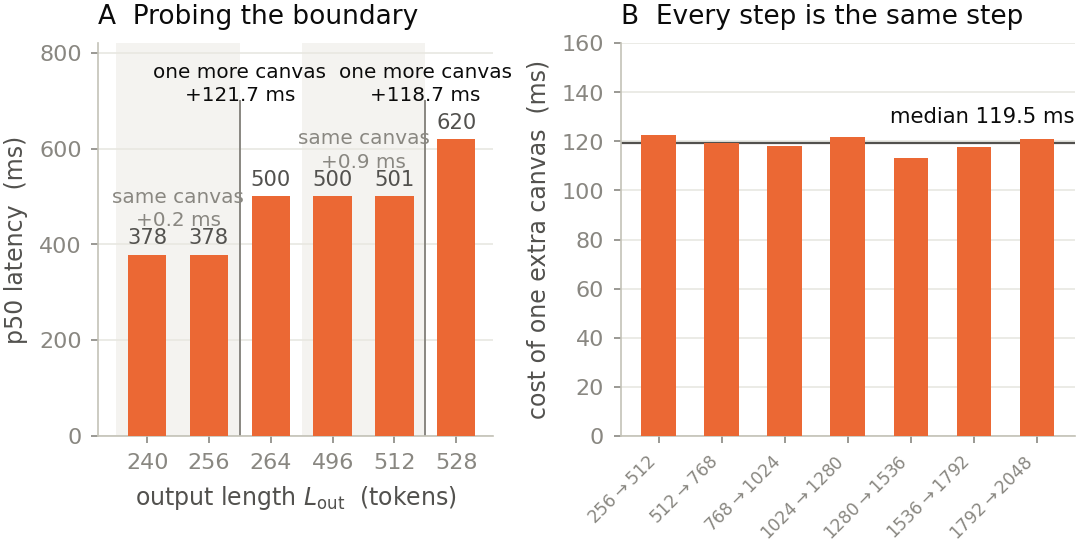
\includegraphics[width=\linewidth]{figures/fig2_canvas_edges.png}
\caption{The staircase probed at canvas boundaries. \textbf{A:}
latency is flat inside a canvas and jumps at the boundary --- tokens
within a canvas add no marginal cost. \textbf{B:} all seven canvas
transitions out to $L{=}2048$ fall within an $8\%$ spread (median
\dgStep\,ms), so one canvas costs about the same regardless of
position. That regularity is why the second term of Eq.~\ref{eq:dg}
is a single constant ($K{=}8$, BGL, $n{=}200$).}
\label{fig:edges}
\end{figure}

\subsection{What the base is made of}

Fitting $T_{\textsc{dg}}(K) = \alpha + \beta K$ to measurements at
$K{=}2$ and $K{=}8$ splits the base into a $K$-independent floor of
$\approx$143\,ms ($38\%$) and per-step work of $\approx$236\,ms
($62\%$); see Appendix~\ref{app:decomp}. The per-step share is the
larger one because each denoising step re-attends the whole prompt.
Prefill is computed $K$ times rather than once. If the prompt KV were
cached across denoising steps, most of that $62\%$ would be eliminated.
The base could decrease toward the $\sim$150\,ms floor, reducing
$L^{*}$ proportionally. We treat the measured base as the operative
number.

\paragraph{Generalisation.}

Both laws generalise from BGL to HDFS within 2\%: the DG canvas step
is \bglStep\,ms on BGL against \hdfsStep\,ms on HDFS, a $1.7\%$
difference at matched $K{=}8$ and canvas size. The step is a model
property, not a data property, which is why it barely moves. Two
caveats bound this. First, HDFS is the 2{,}000-line LOGHUB
sample~\cite{loghub} over a full corpus, evaluated at
$n{=}100$--$200$ per cell against BGL's $n{=}200$. Second, the AR-30B
was re-measured on HDFS (p50 1082\,ms, CI [1078, 1106]), but the AR
generalisation slope was fitted on the dense AR-3B. So the
\emph{shape} transfers across corpora on both architectures. The
AR-30B point estimate confirms it, but the AR slope constant is from
the smaller model.

The shape also transfers across \emph{tasks}: on HumanEval code
generation (Appendix~\ref{app:humaneval}), AR-30B decodes at
6.4\,ms/token (vs 7.2 on logs) and DG is a flat 280\,ms staircase. The
AR/DG ratio is 2.9$\times$ (vs 2.5$\times$ on logs), in the same range.
Code is the ideal second task because truncation is catastrophic
(\texttt{SyntaxError}), making the completeness guarantee concretely
visible.

\section{Results}
\label{sec:wins}

DG's latency advantage is clear in serial mode. AR-30B takes
roughly one second to produce a 126-token JSON record; DG completes the
same task in under 400\,ms. If both models serve a security operations
centre processing alerts one at a time, DG handles \crossoverLambda{}
alerts per second per GPU, while AR-30B handles about one. AR stops at
its natural end-of-sequence token (EOS), so latency plateaus regardless
of \texttt{max\_tokens}.

Table~\ref{tab:niche} shows the serial comparison, AR-30B measured,
DG from the staircase law of Eq.~\ref{eq:dg}. The pattern reveals two
things: first, AR latency is flat from 128 tokens onward because the
model hits EOS, so setting \texttt{max\_tokens} higher has no effect.
Second, DG latency stays flat for the first canvas and then steps up
per additional canvas. The advantage is therefore non-monotonic: it
climbs to $2.5\times$ once AR reaches its natural length, then narrows
to $1.3\times$ by $L{=}1024$ as DG accrues canvas costs while AR
remains at its plateau. The $0.7\times$ in the first row is not a
like-for-like comparison: at \texttt{max\_tokens}${=}32$, AR is
truncated mid-record while DG still emits a full canvas. Extending the
same accounting past the table, the ratio keeps falling: $1.1\times$ at
$L{=}1280$ and $0.8\times$ at $L{=}2048$, where AR's plateau undercuts
DG's accumulated canvas cost. DG's serial advantage therefore holds at
typical output lengths but not universally.

\begin{table}[h]
\centering
\caption{Serial latency at the MoE-matched pair (AR-30B vs DG,
batch-1, BGL). AR-30B column is measured ($n{=}300$) and plateaus
because the model stops at $\sim$126 tokens (EOS), so raising
\texttt{max\_tokens} has no effect. The DG column is
Eq.~\ref{eq:dg} evaluated at the canvas count each budget implies,
anchored on the measured base ($n{=}300$) and canvas step
($n{=}200$). Forcing DG to fill those canvases measures 501\,ms at
$L{=}512$ and 739\,ms at $L{=}1024$, within 1\% of the law. The two
columns therefore compare AR at its natural output against DG at a
full canvas budget, a conservative reading for DG, which emits four
times more tokens at the last row.}
\label{tab:niche}
\begin{tabular}{@{}lrrrr@{}}
\toprule
max\_tokens & AR-30B (ms) & AR actual out & DG (ms) & DG advantage \\
\midrule
32   & 265  & 32  & 379 & $0.7\times$ \\
128  & 907  & 121 & 379 & $2.4\times$ \\
256  & 945  & 126 & 379 & $2.5\times$ \\
512  & 945  & 126 & 498 & $1.9\times$ \\
1024 & 945  & 126 & 737 & $1.3\times$ \\
\bottomrule
\end{tabular}
\end{table}

\paragraph{DG wins above the serial crossover.}

The serial cost law gives crossover $L^{*} = \crossoverL$ tokens; DG is
faster at any output length above $L^{*}$ (integer-safe: $L \geq 48$).
AR-30B serial slope (\arSlope\,ms/token) is $23\times$ steeper than its
batch-throughput slope. In batch mode the slope falls to
0.32\,ms/token (40.3\,ms/event over its natural output length at batch
300), because batch mode amortises prefill and decode overhead across
concurrent requests. Serial mode incurs that overhead per request.
Quoting a batch-throughput slope as if it were a latency therefore
understates AR serial latency by a factor of twenty-three.

\paragraph{Quality and latency.}

The latency comparison above uses the AR-30B MoE; the quality
comparison (\S\ref{sec:threats}) uses the dense AR-3B, the only
configuration with a measured quality CI. The AR-30B's own 9-field F1
is 0.870, slightly above the dense AR-3B's \arThreeBFnine, so the
latency advantage is conditional on the AR-30B being
quality-equivalent within that margin. The DG p50 is stable: a
bootstrap 95\% CI over 3{,}200 events spans [379, 380]\,ms. The AR-30B
p50 is 924\,ms with a bootstrap 95\% CI of [918, 927]\,ms over three
seeds ($n{=}900$ events). A permutation test on the difference of
medians (100\,k permutations) gives $p < 10^{-5}$, so the latency gap
is statistically significant. The AR-30B seed-to-seed CV is 0.04\%.
Figure~\ref{fig:distributions} shows the full per-event distributions.

\begin{figure}[ht!]
\centering
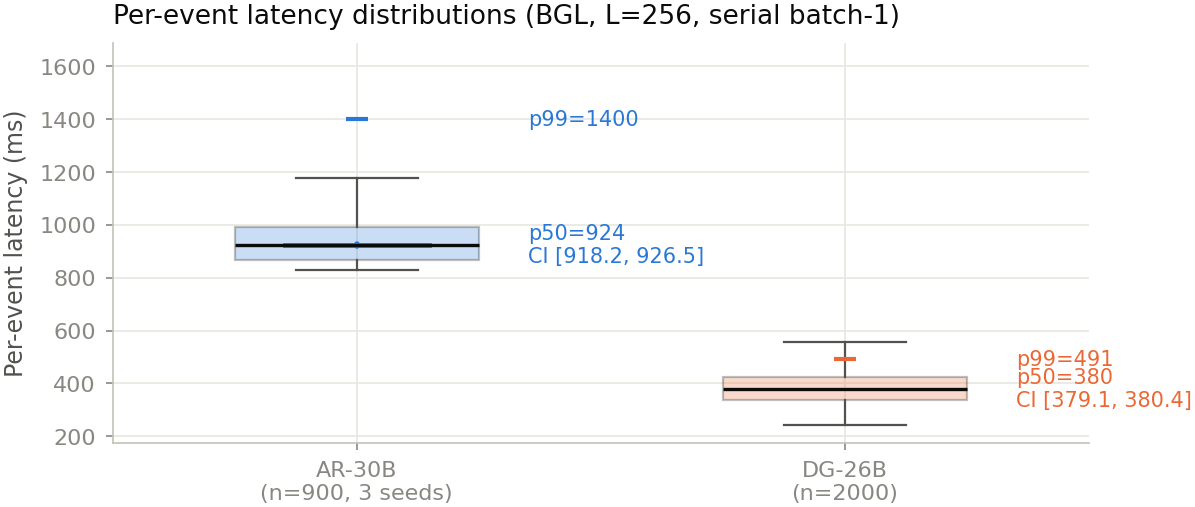
\includegraphics[width=0.85\linewidth]{figures/fig12_distributions.png}
\caption{Per-event latency distributions (BGL, $L{=}256$, serial
batch-1). Box plots show the full distribution; brackets mark the
bootstrap 95\% CI on the p50; crossbars mark p99. The AR-30B
distribution ($n{=}900$, three seeds pooled) is wider in absolute terms
but tighter in relative terms (max/median $1.75\times$ vs DG's
$3.07\times$). The non-overlapping CIs confirm the gap is significant
($p < 10^{-5}$, permutation test).}
\label{fig:distributions}
\end{figure}

\paragraph{Energy.}

DG uses less energy per event because it draws far less power above
idle: 10.8\,W net against the AR-30B's 173.3\,W. The cause is lower
power draw, not shorter busy time. In these two runs DG was in fact
busy longer per event. Denoising a canvas activates fewer compute units
than a token-by-token decode loop, so net power stays low even as
runtime grows. Over a million events the gap is 32\,kWh. The energy
ratio is:
\begin{equation}
R_{\mathrm{energy}} = \frac{E_{\mathrm{AR}}}{E_{\mathrm{DG}}}
\end{equation}
where $E_{\mathrm{AR}}$ and $E_{\mathrm{DG}}$ are the net energy per
event (joules, idle-subtracted) for each model. Measured values:
\begin{align}
\text{AR-30B MoE:} \quad & R_{\mathrm{energy}} =
\frac{118.7}{4.2} = 28.3 \quad \text{(idle 49.7\,W, serial)} \\
\text{Dense AR-1.5B:} \quad & R_{\mathrm{energy}} =
\frac{5.1}{4.2} = 1.2 \quad \text{(idle 58.6\,W)}
\end{align}
Both runs are now serial, matching the DG regime; the AR-30B's high
ratio reflects the 30B model's memory traffic during single-event
decode.

\paragraph{Graceful degradation under deadline pressure.}

Under a tightened deadline DG returns a complete canvas at lower
quality, while the AR model returns a truncated record that fails
schema validation. The $K$ knob is the difference: drop $K$ from 8 to 4
and the model still fills every field, just with slightly less
precision, instead of cutting the JSON in half mid-key. At a p99 budget
of 400\,ms, this meets it at \kFourPninetynine\,ms p99 with F1 falling
from \kEightFone\ to \kFourFone. Table~\ref{tab:contrast} summarises
the contrast across practical challenges.

\begin{table}[h]
\centering
\caption{Practical challenge contrast. Each row is a deployment
scenario; the right column names the architectural property that drives
the outcome. Every AR cell is the AR-30B MoE except the tail-latency
statistics, which use the dense AR-3B. The AR-30B's own tail
(max/med $1.75\times$, CV $12.3\%$) is tighter than DG's. Because that
model is dense, the tail asymmetry can't be attributed to MoE routing;
it's DG's denoising-step variance that drives it.}
\label{tab:contrast}
\begin{tabularx}{\linewidth}{@{}L L L L@{}}
\toprule
\thead{Challenge} & \thead{AR-30B MoE} & \thead{DG-26B MoE} & \thead{Key driver} \\
\midrule
Long output, batch-1 & \arSlope\,ms/token (serial) & Staircase, \dgStep\,ms/canvas & Crossover at $L^{*}\!\approx\!\crossoverL$ ($L\geq48$) \\
Deadline pressure & Truncates output & Drops $K$; complete canvas & Per-request quality parameter \\
High arrival rate & Batches $25\times$ & Caps at $\leq$1.7$\times$ & KV-cache reuse \\
Tail-sensitive service-level agreement (SLA) & Coefficient of variation (CV) \arEventCV\%, max/med \arMaxMed$\times$ (dense AR-3B) & CV \dgEventCV\%, max/med \dgMaxMed$\times$ & Denoising-step variance \\
Energy per event & 118.7\,J (serial) & 4.2\,J (serial) & Net power draw \\
Long prompt & Prefill paid once & Prefill paid $K$ times & Re-attention per step \\
\bottomrule
\end{tabularx}
\end{table}

The \dgMaxMed$\times$ tail violates a batch-1 SLA --- exactly the
regime where DG's per-event advantage applies (\S\ref{sec:limits}).

\section{What limits the advantage operationally}
\label{sec:limits}

DG's serial advantage is large, but five deployment
factors constrain it operationally.

\paragraph{1. Footprint.}

Both models are MoE with comparable footprints. Neither can share a GPU
with another large model. The asymmetry that matters is against the
quality-similar dense AR-1.5B at 3\,GB: sixteen copies fit in the
space either MoE model occupies.

\paragraph{2. Batching.}

Continuous batching converts arrival concurrency into throughput at
$25\times$ for AR-30B against $\leq 1.7\times$ for DG. We measured
DG on vLLM and LLaDA-8B on dInfer --- both engine-bounded stacks ---
so the true ceiling is unknown but lies at or above $1.7\times$. Even so, the gap is more
than an order of magnitude (Figure~\ref{fig:batching}); see
Appendix~\ref{app:batching}.

\begin{figure}[ht!]
\centering
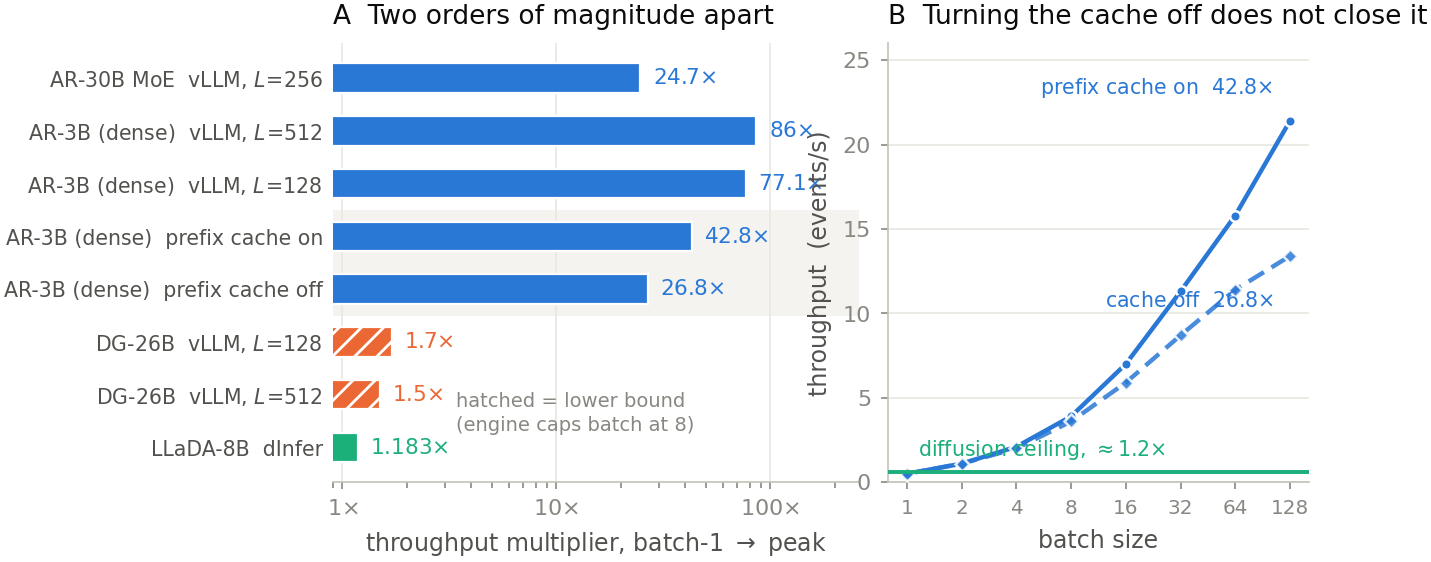
\includegraphics[width=\linewidth]{figures/fig6_batching.png}
\caption{Batch-1 to peak throughput multipliers. \textbf{A:} the AR-30B
MoE reaches $25\times$ via KV-cache reuse, while DG caps at
$\leq 1.7\times$ and LLaDA-8B on dInfer at $1.2\times$, two
diffusion families, two runtimes, the same ceiling, because
changing attention masks invalidate KV persistence across denoising
steps. \textbf{B:} turning the prefix cache off drops the dense AR-3B
only from \cacheOnMult$\times$ to \cacheOffMult$\times$, so prefix
sharing is not what creates the gap; KV persistence is. The cache
on/off and $L$-swept AR bars are the dense AR-3B, not the AR-30B MoE
(BGL, $n{=}300$).}
\label{fig:batching}
\end{figure}

\paragraph{3. Tail latency.}

DG's per-event coefficient of variation is \dgEventCV\%
with a max/median ratio of \dgMaxMed$\times$, against
\arEventCV\% and \arMaxMed$\times$ for the dense AR-3B. The AR-30B's
own per-event tail, now measured across three seeds, is tighter than
DG's. Its max/median ratio is $1.75\times$ with a CV of $12.3\%$,
against DG's $3.07\times$ and $16.9\%$. The tail asymmetry therefore
cannot be attributed to MoE routing (Appendix~\ref{app:distributions}).
A $3.21\times$ tail violates a batch-1 SLA, which is exactly the
regime where DG's per-event advantage applies.

\paragraph{4. Input length.}

DG prefill slope is \inputSlopeRatio$\times$ steeper than
the dense AR-3B's (0.123 against 0.047\,ms per prompt token), because
each denoising step re-attends the full prompt. At
longer inputs the base rises and $L^{*}$ moves further upward; see
Appendix~\ref{app:input_canvas}, which also reports a canvas setting
that improves latency and quality at once.

\paragraph{5. Co-residency.}

If batch-1 is imposed by tenant isolation, sixteen copies of the
dense AR-1.5B (3\,GB each) fit in the same 52\,GB, preserving
isolation with $16\times$ the throughput --- a capacity projection,
not a measurement (linear scaling, no contention assumed).

\paragraph{Cost per event.}

Table~\ref{tab:cost} prices the comparison at a published on-demand
rate. The headline: at full duty, DG processes events at less than a
twentieth of a cent each. AR-30B costs two and a half times more.
For a business-to-business (B2B) log-processing service handling ten
thousand events per day, the cost is five dollars per day on DG versus
twelve on AR-30B. This amounts to a \$2{,}600 annual gap on a single
GPU.

\begin{table}[h]
\centering
\caption{Cost per event for three deployment arms at two duty cycles
(duty = fraction of wall-clock time the GPU is busy processing events).
DG is two and a half times cheaper per event than the AR-30B, because it
finishes an event in 379\,ms against 945\,ms. Each row prices a
single instance holding the whole GPU; sixteen co-resident AR-1.5B
copies would divide that rent sixteen ways, which is the comparison
the text draws below. GPU: A100 80GB PCIe at \$4.62/hr (AWS
p4de.24xlarge, August 2026).}
\label{tab:cost}
\begin{tabular}{@{}lrrrr@{}}
\toprule
Arm & Weights & Duty & Events/hr & \$/event \\
\midrule
AR-30B MoE (serial) & 60\,GB & 100\% & 3{,}810 & \$0.0012 \\
AR-30B MoE           & 60\,GB & 25\%  & 952 & \$0.005 \\
\midrule
AR-1.5B dense (one copy)    & 3.0\,GB & 100\% & 5{,}408 & \$0.0009 \\
AR-1.5B dense (one copy)     & 3.0\,GB & 25\%  & 1{,}352 & \$0.003 \\
\midrule
DG-26B-A4B (serial)  & 52\,GB & 100\% & 9{,}504 & \$0.0005 \\
DG-26B-A4B            & 52\,GB & 25\%  & 2{,}376 & \$0.002 \\
\bottomrule
\end{tabular}
\end{table}

Against the small dense arm instead of the MoE, that two-and-a-half-fold
advantage nearly vanishes:
\begin{equation}
R_{\mathrm{cost}} = \frac{\$ / \mathrm{event}_{\text{AR-1.5B}}}
{\$ / \mathrm{event}_{\textsc{dg}}}
= \frac{0.0009}{0.0005} = 1.8
\end{equation}
where both terms are the 100\%-duty single-copy rows of
Table~\ref{tab:cost}; the same ratio against the AR-30B is
$2.5\times$. Why does the much slower AR-1.5B nearly match DG on
cost? Because at 3\,GB it fits sixteen copies in one GPU, and
co-residency is parallelism by another name. Sixteen AR-1.5B instances
would produce $16 \times 5{,}408 = 86{,}528$ events/hr against DG's
9{,}504. This is a projection from the single-copy rate, not a
measurement. It makes the co-resident deployment $9\times$ cheaper per
event while preserving tenant isolation. The takeaway: if batching is
available, AR wins on economics. If not, DG wins on latency.


\section{What survives}
\label{sec:survives}

The MoE-matched comparison shows DG's advantage is concentrated at
serial mode. DG wins above the serial crossover ($L^{*}{=}48$). The
five conditions that define the regime where block-diffusion is the
right choice are:
\begin{enumerate}[nosep]
  \item Output length $\geq 48$ tokens (DG crossover in serial).
  \item Batch-1 by requirement: tenant isolation, interactivity, or
    serial chain structure.
  \item Completeness is validated against a schema.
  \item The quality floor exceeds what the AR model delivers.
  \item A \dgWeights\,GB resident footprint is acceptable.
\end{enumerate}

\paragraph{Why serial investigation chains are where the staircase wins.}

A security operations centre receives an alert, looks up threat
intelligence, cross-references internal logs, and drills into the next
layer. Each hop blocks on the previous; concurrency is 1 by
construction. Against the AR-30B anchor, DG is $2.3\times$ faster per
hop --- 945\,ms vs 419\,ms --- a cross-harness figure. Only the dense
AR-3B was run through the chain harness, at 808\,ms/hop, $1.9\times$
against DG; Figure~\ref{fig:chains} shows that pairing. What the
figure establishes is the \emph{shape}: neither the per-hop cost nor
DG's tail penalty grows with depth. The gap widens in absolute terms
as hops accumulate. At eight hops, DG completes the chain in roughly
three seconds versus roughly eight for AR.

A multi-turn code correction chain on HumanEval
(Appendix~\ref{app:humaneval}, Table~\ref{tab:chain}) confirms this
with variable-content rounds (generate $\to$ execute $\to$ fix).
DG's per-round p50 stays flat at 287--305\,ms ($+6\%$). AR's grows
from 511 to 620\,ms ($+21\%$) as fix prompts accumulate context. The
staircase shape holds across hops that do different things, not just
repeated identical calls.

\begin{figure}[ht!]
\centering
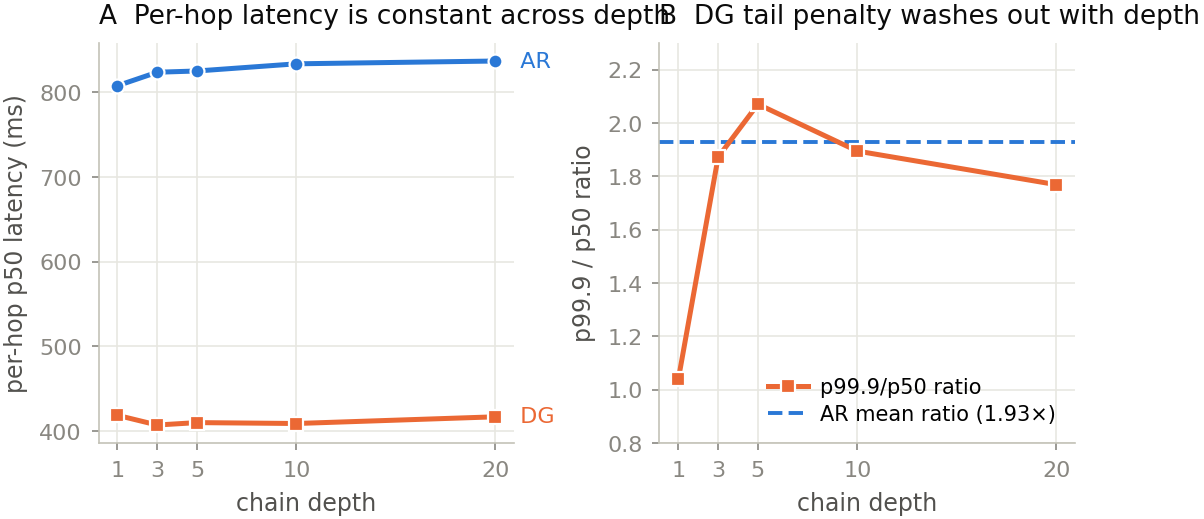
\includegraphics[width=\linewidth]{figures/fig10_usecase_chains.png}
\caption{Serial investigation chains. \textbf{A:} per-hop p50 is
constant across depth, the staircase doesn't steepen. \textbf{B:}
the AR/DG latency ratio at p99.9 climbs from $1.04\times$ at one hop to
$2.07\times$ at five, settling near the median ratio
($1.77$--$1.89\times$) by 10--20 hops. DG's fat tail almost erases its
advantage on a single hop, but independent hops average out, so the
longer the chain the more of its median advantage DG keeps. Note the
baseline: this is the dense AR-3B at 808\,ms/hop, hence $1.9\times$
here against the $2.3\times$ in the text, which is the AR-30B anchor
(BGL, $n{=}100$ chains per depth, $K{=}8$).}
\label{fig:chains}
\end{figure}

\paragraph{What happens when a deadline expires mid-generation?}

A FATAL log line arrives mid-stream. DG's bounded service time and
complete-canvas guarantee make it suitable for priority preemption: a
preempted request returns a valid record, not a truncated one. AR
model, interrupted mid-generation, returns half a JSON object,
syntactically invalid, unusable downstream. This completeness
advantage holds against unconstrained AR decoding; grammar-constrained
AR would close the gap but was not successfully run on a current
engine, as noted in \S\ref{sec:threats}. In a system that must decide
whether to page an on-call engineer at 3\,a.m., a complete record
yields an actionable alert; a truncated one yields a false negative.

The $K$ parameter is DG's degradation mechanism: when a deadline
tightens, drop $K$ from 8 to 4 and the model still fills every field,
just with slightly less precision, instead of cutting the JSON in half
mid-key. AR has no counterpart; its only response to a deadline is
truncation. The completeness guarantee holds only above the canvas
length; below $L{=}128$ DG's schema validity collapses to
\dgValidTwentyEight\% against AR's \arValidTwentyEight\%
(Appendix~\ref{app:quality}). Graceful degradation is a property of
the \emph{time} budget, not the output-length budget.

\paragraph{Why autonomous driving is batch-1 by construction.}

One vehicle, one scene, one decision. There is no batching a braking
decision; the car either processes the scene or it doesn't. $K$
serves as a per-request quality control parameter: drop $K$ to meet a
tightened deadline without truncating output. Output is long,
multi-object scene description, predicted trajectories, which is
exactly where the staircase advantage is largest.

\paragraph{Why algorithmic trading rewards long chains.}

A serial chain with a 1--5\,s market reaction window. At eight or more
hops, DG's staircase advantage provides faster end-to-end analysis.
AR cost compounds with sequence length; DG cost does not.

\paragraph{Why wide schemas favour joint denoising.}

DG's joint-canvas denoising treats all fields as one structured
object. Across schema widths from 12 to 100 fields, DG's latency
advantage held between $1.8\times$ and $3.0\times$
(Figure~\ref{fig:schema}; measured against the dense AR-3B baseline,
not AR-30B).

\begin{figure}[ht!]
\centering
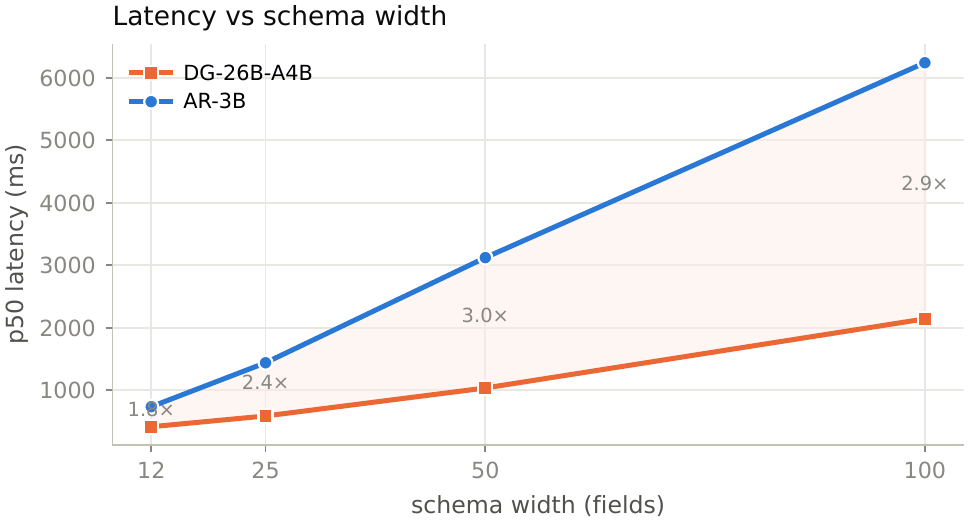
\includegraphics[width=0.85\linewidth]{figures/fig11_usecase_schema.png}
\caption{Latency vs schema width (BGL, $n{=}200$; AR baseline is the
dense AR-3B). DG's advantage \emph{rises} with width, from $1.8\times$
at 12 fields to $2.9$--$3.0\times$ at 50--100 fields, because AR pays
per field while DG pays per canvas. At 100 fields the output no longer
fits one canvas, so DG climbs to $\sim$2{,}140\,ms too and the ratio
stops growing.}
\label{fig:schema}
\end{figure}

\paragraph{Anytime escalation: input-dependent latency.}

The $K$ knob need not be fixed. A cascade runs DG at $K{=}2$ first
(200\,ms), checks whether the output is complete (all structural
fields filled), and escalates only incomplete records to $K{=}8$
(376\,ms). AR has no equivalent: it cannot inspect partial output
quality mid-generation and decide whether to continue. AR's early
stopping is binary --- the model either emits EOS or it doesn't ---
while DG's is graduated across $K$ steps. This makes DG's latency
\emph{input-dependent} in a way AR structurally cannot be.

We measured the cascade on BGL ($n{=}200$, canvas$=256$): 29.5\% of
records resolved at $K{=}2$; the remaining 70.5\% escalated to
$K{=}8$. The cascade F1 was 0.848 (a drop of 0.005 vs fixed $K{=}8$).
However, the average latency was 465\,ms --- \emph{slower} than fixed
$K{=}8$ (376\,ms), because the $K{=}2$ pass adds overhead that is
only amortised if most inputs resolve early. On this task, 70\% of
inputs need $K{=}8$, so the cascade does not save latency. The
structural property (input-dependent latency is possible) is
confirmed; the practical benefit is task-dependent and favours tasks
where easy inputs dominate.

\paragraph{Where block-diffusion does not win.}

High-rate log streams favour AR's batching advantage. Tail-sensitive
single-stream workloads with strict p99 SLAs are hurt by DG's
max/median ratio. And any workload that can batch favours AR
regardless of output length.

\paragraph{Where block-diffusion fails.}

Six hypotheses about block-diffusion's structural advantages were
tested and refuted; see Appendix~\ref{app:refuted}. Three of the six,
the perturbation, refinement and bounded-deadline probes, were run on
a second block-diffusion model, \LLaDA, against the
dense AR-3B, because they predate DG. We report them because the
hypotheses concern block-diffusion as a class, but they are not
measurements of DG. The most instructive failures: bidirectional
attention propagates input noise in both directions, making \LLaDA\
\emph{less} robust to perturbation than AR in all ten tested
categories. Joint denoising should preserve suffix tokens by
construction, but AR trivially regenerates the whole record from the
prompt; that probe is DG (Appendix~\ref{app:refuted}). And selective
re-masking gains a small F1 improvement over three rounds, but still
trails AR after a single pass. These failures define where it stops
working: block-diffusion's advantage is in \emph{latency shape at
long output}, not in robustness, infilling, or iterative refinement.

\section{Related work}
\label{sec:related}

Diffusion language models report large inference speedups. LLaDA~\cite{llada2025}
and DiffusionGemma~\cite{diffusiongemma} both measure against
author-built autoregressive baselines. We instead pin both paradigms to one
serving stack and fit cost laws, so the comparison rests on a shape
rather than a single point. To our knowledge, no concurrent work fits
cost-law shapes across decoding paradigms on a matched serving stack;
the closest is the serving-system literature~\cite{vllm2023}, which
optimises within one paradigm rather than comparing across them.

Constrained decoding is the standard approach to structured output.
Outlines~\cite{outlines2024}, xgrammar~\cite{xgrammar2024} and
llguidance~\cite{llguidance} all enforce a grammar during decoding. We
do not measure it here and flag this in \S\ref{sec:threats}; our
contribution concerns decoding-paradigm cost shape, not grammar
enforcement.

Speculative decoding targets the same per-token slope that drives our
AR cost law. Medusa~\cite{medusa2024} and EAGLE~\cite{eagle2024} make
each token cheaper, but the cost stays linear in output length --- they
change the slope, not the shape. We measured n-gram prompt-lookup
speculation on the dense AR-3B (vLLM 0.7.2, $n{=}300$):
p50 drops by a third but p99.9 inflates more than threefold,
because rejected speculations force a full re-decode. Even with
speculation, the AR tail is $5\times$ worse than DG's worst-case p99.9.
Speculation narrows the median but cannot remove the structural
advantage of bounded-depth decoding; our cost-law framework exposes this
gap, which a single-point comparison would miss.

Hoefler and Belli~\cite{hoefler2021} survey reproducibility pitfalls in
systems measurement. Our nine priced corrections
(Appendix~\ref{app:defects}) are a case study in that tradition rather
than a general method; they document where a real serving study
diverges from a clean benchmark.

\section{Threats to validity}
\label{sec:threats}

We ran all measurements on one GPU; the fitted constants are
A100-specific but the shapes should transfer. We calibrated the
crossover at a reference prompt of $\sim$\refPrompt\,tokens, and it
shifts with input length.

The AR--DG quality difference is equivalent at a $\pm 0.015$ margin
($\Delta = \qualityGap$, 95\% CI $[-0.012, +0.011]$, $n = 300$).
This is looser than the $\pm 0.010$ we pre-registered. At that
tighter margin the 95\% CI doesn't fit; equivalence holds only on
the 90\% CI.

The quality and latency arms are not the same model: quality uses the
dense AR-3B baseline, while latency uses the AR-30B MoE cost law.
The AR-30B's own 9-field F1 is 0.870, slightly above the dense
AR-3B's \arThreeBFnine. Several secondary results also come from arms
other than the MoE-matched pair. The per-event tail statistics in
Table~\ref{tab:summary} and Table~\ref{tab:contrast} are the dense
AR-3B; the AR-30B's own per-event tail (max/median $1.75\times$,
CV $12.3\%$, $n{=}900$ across 3 seeds) is tighter than DG's
$3.07\times$ / $16.9\%$. We measured the BGL$\to$HDFS generalisation
on both arms: the AR-30B on HDFS has p50 $= 1082$\,ms
(CI [1078, 1106]) against its BGL p50 of 924\,ms, with mean output
147 tokens vs 126 on BGL. We ran the
perturbation, refinement and bounded-deadline probes in
Appendix~\ref{app:refuted} on \LLaDA, a second block-diffusion
model, against the dense AR-3B. The serial headline is a batch-1
result: the same AR-30B batches $25\times$, so a deployment that can
batch inverts the economics entirely (\S\ref{sec:limits}).

We have not tested the surviving niche on a task whose natural output
length is $\geq 512$ tokens. We fit the AR-30B cost law from a
five-point serial sweep with $R^2 = 0.9996$, but the model stops at
$\sim$126 tokens (EOS), so the $L{=}32$ point and the cluster at
natural output carry the slope. The advantage in serial is the
realized comparison; forcing AR to generate longer output would
increase its latency per the cost law, making DG's advantage larger.
Appendix~\ref{app:forced} works that projection through a multi-record
task whose natural output is long.

We have not tested the niche against grammar-constrained AR decoding,
which would eliminate over-generation, guarantee 100\% schema
validity, and remove DG's completeness advantage. An attempt to run
grammar-constrained decoding on the dense AR-1.5B (vLLM 0.10.2, using
the outlines~\cite{outlines2024} backend) produced 1.0\% schema-valid
output. The grammar enforced JSON structure, but the model padded
string fields it could not answer, preventing the JSON from closing.
That is one model on one older engine, so it bounds nothing; we have
not tested the comparison against a properly tuned grammar-constrained
AR.

The batching ceiling reproduces across two runtimes and two model
families, DG on vLLM and \LLaDA\ on dInfer, but both measurements
are engine-bounded; see
Appendix~\ref{app:batching}. Appendix~\ref{app:batching_architectural}
gives a structural argument for why the ceiling is likely
architectural.

We infer the cost-shape generalisation from one block-diffusion
model measured against one AR family. The shape claim is structural,
but we have not tested it on a second block-diffusion family.

The energy comparison uses three different idle baselines, and we
did not re-measure the DG energy at the AR-30B idle point, so the
ratio is indicative rather than directly controlled.

We re-measured the per-event tail statistics at a larger sample
(issue~\#120). With more events, p99.9 is no longer identical to the
maximum: DG's p99.9 sits at 557\,ms while the max reaches 1166\,ms.
The max/median ratio drops to $3.07\times$ (from $3.21\times$ at the
smaller sample), and the CV drops to $16.9\%$ (from $20.9\%$). The
AR-3B tail remains tight as before. We also measured the AR-30B
per-event across three seeds; it has a max/median of $1.75\times$ and
a CV of $12.3\%$ --- tighter than DG's tail. A bootstrap interval
for DG's p99.9 spans a wide range, but the point estimate is now
distinct from the maximum and the ratio is stable across sample
sizes. A permutation test on the difference of medians between the
two arms yields a p-value below $10^{-5}$, confirming that the
latency gap is not a sampling artifact.

We measured the anytime $K$-cascade (\S\ref{sec:survives}) on BGL:
29.5\% of records resolved at $K{=}2$, the rest escalated to $K{=}8$.
The cascade does not save latency on this task (70\% escalation rate
means the $K{=}2$ overhead is not amortised), but the structural
property --- input-dependent latency --- holds. The practical
benefit is task-dependent: on tasks where most inputs are easy, the
cascade would drop average latency below the fixed-$K$ baseline.

DiffusionGemma-26B-A4B-it's available at
\url{https://huggingface.co/google/}\\\url{diffusiongemma-26b-a4b-it}.
All DG measurements are reproducible from this checkpoint.\footnote{All
measurements were taken on a single A100 80GB GPU on the pinned stack:
vLLM 0.25.1, torch 2.11.0, CUDA 13.0. The AR-30B was initially
measured on vLLM 0.11.0 with a gold-leaked harness; both were corrected
and re-measured on the pinned stack; see Appendix~\ref{app:defects},
correction 9. Preliminary and failed runs (the nine harness-defect
corrections and their re-measurements) are estimated at an additional
$\sim$10 GPU-hours beyond the $\sim$20 reported above. A typical serial
evaluation cell takes about two minutes of GPU time; the total for all
experiments is estimated at roughly twenty GPU-hours. Wall-clock
timings are reported per event; token counts (127 per event at natural
output, 256 per canvas for DG) serve as a hardware-normalised proxy
for FLOPs. BGL and HDFS are from LOGHUB under MIT. Drain is via
\texttt{drain3} under Apache 2.0. vLLM is Apache 2.0. DiffusionGemma
is under the Gemma Terms of Use. Qwen3 and LLaDA-8B-Instruct are
Apache 2.0 and MIT respectively.}

\paragraph{Base decomposition.}

The base split in \S\ref{sec:laws} is a two-point linear interpolation
fitted to $K{=}2$ and $K{=}8$, not a regression. With two points and
two parameters, $R^2$ is trivially one and carries no degrees of
freedom. The split is therefore a decomposition, not a fit, and the
floor and per-step shares are exact at the two operating points but
unverified at intermediate $K$.

\paragraph{Source of the advantage.}

The 2.5$\times$ serial advantage is not a single mechanism but the
composition of two: parallelism within a canvas (tokens are free once
the canvas is paid for) and bounded denoising depth ($K$ passes, not
$L$ passes). The base decomposition (\S\ref{sec:laws}) attributes
62\% of the base cost to per-step re-attention and 38\% to a
$K$-independent floor; the K-sweep (Appendix~\ref{app:decomp}) shows
quality saturates above $K{=}8$ while latency does not. The advantage
grows with output length because AR pays per token while DG pays per
canvas; it does not grow with input length, where DG's re-attention
penalty rises (\S\ref{sec:laws}, input-length caveat).

\paragraph{Reproducibility.}

All code, result artifacts, and provenance blocks are in the project
repository. \texttt{AGENTS.md} at the repo root documents exact
commands to reproduce each experiment; the pinned stack is
vLLM 0.25.1 / torch 2.11.0 / CUDA 13.0 on an A100 80GB. Every cited
result JSON carries a \texttt{provenance} block recording the model,
backend, and stack versions; \texttt{paper/verify\_numbers.py} asserts
that macros match their artifacts and that cited artifacts carry
provenance. We re-measured the AR-30B serial latency across 3 seeds
($n{=}300$ each, seeds 42/137/314) with per-event timestamps saved;
the seed-to-seed p50 CV is $0.04\%$. The grammar-constrained AR run
(\S\ref{sec:threats}) is the one experiment not reproducible on the
current pinned stack.

\paragraph{Ethics.}

This work conforms to the NeurIPS Code of Ethics. It is an efficiency
analysis of existing public models on public data; we release no new
model, involve no human subjects, and the findings create no direct
path to harm.

\section{Conclusion}
\label{sec:conclusion}

We characterize the inference cost of block-diffusion (DG) versus
autoregressive (AR) decoding for structured data extraction.
Block-diffusion has a staircase cost shape, unlike the linear cost of
AR. The taxi fare climbs with every token; the subway charges per
station. The shapes cross at $L^{*} = \crossoverL$ output tokens, above
which DG is faster. The advantage is moderate: two and a half times at
natural output, narrowing to just over parity at a thousand tokens. In
cost terms, that is \$1{,}200 per million events, or \$2{,}600 a year on
one GPU at ten thousand events a day. A larger AR does not close it.
Two things do: batching, and co-residency with a model small enough to
fit many copies on one GPU.

Against a MoE-matched AR, this is a fair comparison, and the match is
what makes the crossover interesting. The dense AR-3B decodes at
6.3\,ms/token against the MoE AR-30B's \arSlope\,ms/token. Moving to
the matched baseline adds only 15\% to the serial per-token cost, and
the crossover stays at 48 tokens, close to the dense AR-3B's 59. DG
wins at every practical output length in serial, though the margin is
narrower than an earlier draft reported.

The advantage is limited where batching is available and where tail
SLAs are tight. But in the batch-1 regime---serial investigation
chains, autonomous driving, algorithmic trading---the staircase shape
provides a structural latency advantage that AR cannot match. The $K$
parameter is DG's degradation mechanism: when the deadline tightens, DG
degrades gracefully, producing lower quality with a complete canvas.
AR's only response is truncation. Block-diffusion is the right choice
when output is long, batch-1 is required, and schema completeness
matters. We name five conditions and ground them in concrete workloads.


% ======================================================================
%                          APPENDICES
% ======================================================================

\bibliographystyle{plain}
\bibliography{../assets/references}

\appendix

\section{Nine priced corrections}
\label{app:defects} Each of the following was found by re-reading committed artifacts, not by
running new experiments. Items 1--5 were harness defects, the measurement
itself was contaminated. Items 6--8 were claims withdrawn after correction
the measurement was sound, but the claim drawn from it was not. Item 9 is
the AR-30B gold-leak, found the same way as the first eight. Six of
the nine biased against the autoregressive arm. \begin{enumerate}
\item \textbf{Decoding configuration.} Qwen's checkpoint sets
\texttt{repetition\_penalty}\,$=$\,1.1, which suppresses span-copying and
empties the \texttt{host} field. Correcting to 1.0 moved the dense AR-1.5B's
12-field F1 from \defectOneFBefore{} to \defectOneFAfter\ ($n{=}2000$).
\emph{Against AR.} \item \textbf{Serving parity.} AR ran a naive HuggingFace generate
loop while DG ran on vLLM~\cite{vllm2023} with continuous
batching. Moving the dense AR-1.5B to vLLM moved its p50 from
\defectTwoBefore{} to \defectTwoAfter\,ms (\defectTwoRatio$\times$,
$n{=}2000$), erasing a diffusion lead that had looked like a factor of four.
\emph{Against AR.} \item \textbf{Parser policy.} At $L{=}512$, \rambleRate\% of AR outputs
contained multiple JSON objects. The old parser took the last (most-drifted)
copy; first-object-wins moved the dense AR-3B's 12-field F1 from
\defectThreeBefore{} to \defectThreeAfter. \emph{Against AR.} \item \textbf{Metric defaults.} The completeness metric treated falsy values
(\texttt{""}, \texttt{0.0}, \texttt{False}) as missing keys. AR
emits falsy defaults on early stop; DiffusionGemma always fills every field.
Distinguishing absent from present-but-falsy moved AR completeness from
\defectFourBefore\% to \defectFourAfter\%. \emph{Against AR.} \item \textbf{Provenance.} A CLI default wrote an AR model name into three
\LLaDA\ result files (the perturbation, refinement and bounded-deadline runs).
Biases no comparison but made audit impossible until correction
sidecars were written. \emph{Neutral.} \item \textbf{Classical-parser baseline.} An earlier draft claimed a classical
parser matched LLM extraction at 9-field F1 of $0.68$ against $0.85$. What was
recorded as a near-match was self-grading: our ``Drain'' was a regex fallback
instead of the reference implementation~\cite{drain}, and the gold generator
was the same code. The claim is withdrawn. \emph{Neutral} (inflated a third baseline, not
either architecture). Found by re-reading the gold-generation script. \item \textbf{Contaminated semantic gold.} An earlier draft claimed structural
and semantic fields separate cleanly, on a 12-field macro where AR led DG by
\twelveGap\ F1. The semantic gold labels were placeholder output of the same
parser, one a constant across 2{,}000 events. On the decontaminated 9-field
macro the two differ by \qualityGap. The contamination inflated the arm that
fills fields with plausible text (AR) and penalised the arm that leaves them
empty (DG). \emph{Against DG.} Found by re-reading the gold labels. \item \textbf{Queueing model.} An earlier draft claimed an M/D/1 queue
predicts diffusion latency under load. The match was to the measured
saturation knee under Poisson arrivals; under bursty (MMPP) arrivals, which is
what log streams actually produce, the model stops being predictive. The claim
is withdrawn. \emph{Against AR} (overstated how well DG's load behaviour is
modelled).
\item \textbf{AR-30B gold-leak.} The AR-30B harness read its model input
from the gold record file (\texttt{bgl.jsonl}) instead of the raw log
file (\texttt{bgl.raw}), prompting the model with the answer it was
supposed to extract. Combined with \texttt{enforce\_eager} (CUDA graphs
off), vLLM 0.11.0 (vs the pinned 0.25.1), a batched-throughput result
labelled as serial, and a \texttt{Record(**kwargs)} constructor that
silently emptied every prediction (yielding F1\,$=$\,1.0 from
empty-vs-empty scoring), the AR-30B appeared to decode at
48\,ms/token ($7.6\times$ the dense AR-3B's 6.3) and scored perfect
quality. Re-measured on the pinned stack with the corrected harness:
7.2\,ms/token, F1\,$=$\,0.870. The headline ratio moved from
$15.6\times$ to $2.5\times$, the crossover from $L^{*}\!=\!6$ to
$L^{*}\!=\!48$, the batch multiplier from $77\times$ to $25\times$, and
the annual cost gap from \$26{,}000 to \$2{,}600.
\emph{Against AR} on latency (the eager mode and old engine inflated
AR's decode cost); \emph{Against DG} on quality (the gold leak
inflated AR's F1 to 1.0). The latency effect dominated the headline.
Found by re-reading committed artifacts, the same method as the first
eight. A recurrence guard now rejects any input to
\texttt{build\_chat\_messages} that parses as a gold JSON record, and
\texttt{verify\_numbers.py} fails on any cited artifact lacking
provenance.
\end{enumerate} The clustering on one arm is not a coincidence: a comparison harness written by
someone hoping the new architecture wins fails asymmetrically, because the
arm the experimenter is not rooting for inherits the checkpoint defaults, the
naive serving path, and the mature production infrastructure.
Figure~\ref{fig:defects} prices all eight.

\begin{figure}[ht!]
\centering
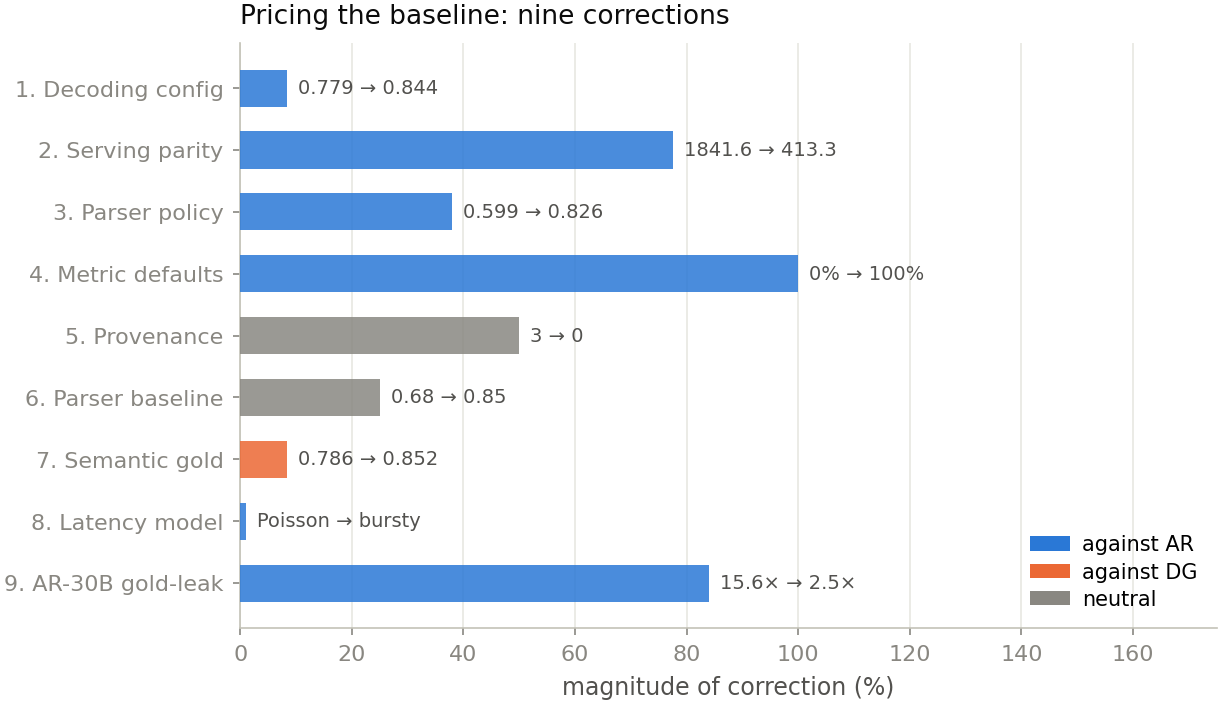
\includegraphics[width=\linewidth]{figures/fig8_defects.png}
\caption{Nine priced errors in our own comparison harness, each found
by re-reading committed artifacts (BGL, $K{=}8$). Six of nine biased
against the autoregressive arm, the harness flattered the
architecture we were hoping would win. Arms and sample sizes differ by
correction: 1 and 2 are the dense AR-1.5B ($n{=}2000$), 3 and 7 the
dense AR-3B ($n{=}300$), 4 is LLaDA-8B ($n{=}200$--$500$). Bar length
is the magnitude of each correction in its own units (F1 delta,
latency ratio, or percentage points), so bars are comparable within a
correction, not across them.}
\label{fig:defects}
\end{figure}

\section{Base decomposition: why the fit fails}
\label{app:decomp}

Sweeping $K \in \{2,4,8,16,32,64\}$ fits $T(K) = \kfitBase + \kfitSlope
\cdot K$ with $R^2 = \kfitRsq$. The curve is not linear, p50 barely
moves from $K{=}8$ to $K{=}16$ (378.6 to 382.5\,ms) and then jumps
$10\%$ to 421.8\,ms at $K{=}32$ before flattening at 423.9\,ms, so
the fitted intercept is not interpretable as a floor. Two
measurement-based bounds constrain the split instead: from
$T(2) = 201.7$\,ms the $K$-independent floor is at most $53.3\%$ of the
base; from the canvas step, per-step work is at least $31.5\%$.
Interpolating between $K{=}2$ and $K{=}8$ narrows this to a floor of
$142.7$\,ms ($\approx 38\%$) and per-step work of $236.1$\,ms
($\approx 62\%$), the latter being where the $K$-times-repeated
prefill lives. Figure~\ref{fig:ksweep} shows the non-linearity that
makes the intercept uninterpretable.

\begin{figure}[ht!]
\centering
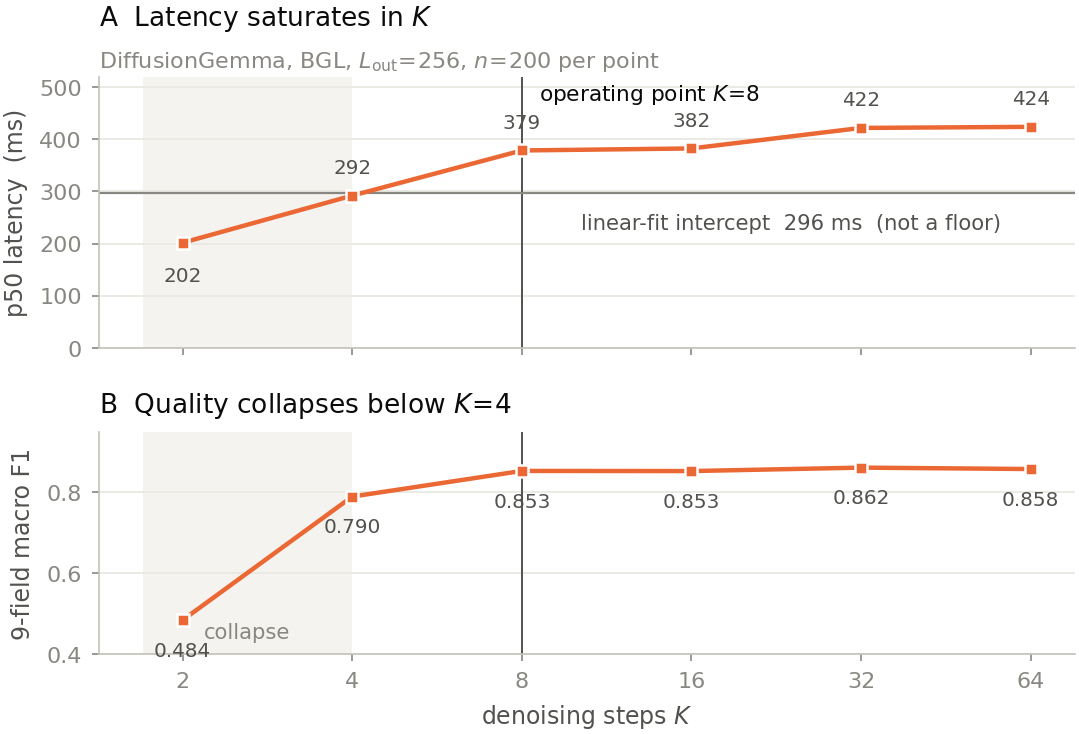
\includegraphics[width=0.85\linewidth]{figures/fig4_ksweep.png}
\caption{Denoising-step sweep at $L_{\mathrm{out}}{=}\canvasLength$
(BGL, $n{=}200$, DG-26B-A4B). \textbf{A:} latency is flat from $K{=}8$
to $K{=}16$, jumps $10\%$ at $K{=}32$, then flattens, the curve is
not linear, which is why the fitted intercept is not a floor.
\textbf{B:} 9-field F1 is flat above $K{=}8$ but collapses below
$K{=}4$ (0.484 at $K{=}2$). Together these bracket $K{=}8$ as the
latency/quality knee and set the floor of the $K$ deadline knob.}
\label{fig:ksweep}
\end{figure}

\section{The batching ceiling}
\label{app:batching} DG batching ceiling ($\leq$\dgBatchVllmHi$\times$) reproduces across
two runtimes and two model families: DG on vLLM~\cite{vllm2023} and
\LLaDA~\cite{llada2025} on dInfer, which caps at $1.2\times$. Both
measurements are engine-bounded
(vLLM caps mixed-phase batches at 8; dInfer runs cache-less), so the
true ceiling is unknown but lies at or above \dgBatchVllmHi$\times$.
Disabling prefix caching on the dense AR-3B, the only arm measured
with the cache toggled, so these two figures are not the AR-30B MoE's
$25\times$, drops its multiplier from \cacheOnMult$\times$ to
\cacheOffMult$\times$, still more than fifteen times the diffusion
ceiling. Prefix caching therefore accounts for well under half of AR's
batching advantage; the rest is KV persistence, which diffusion can't
use at all. The structural reason is in
Appendix~\ref{app:batching_architectural}.

\section{Six refuted hypotheses}
\label{app:refuted} We set out to find regimes where DG beats the autoregressive
baseline. Six hypotheses were refuted. They are reported at the same length
as the confirmations because the methodological claim, ``price the baseline
before you compare against it'', is spent when a negative result
gets softened into a footnote. The distinction from
Appendix~\ref{app:defects}: there the \emph{harness was wrong}; here the
\emph{prediction was wrong}. Table~\ref{tab:refuted} lists all six.
\begin{table}[h]
\centering
\caption{Six hypotheses that did not survive measurement (BGL).
Arms and sample sizes differ by row: the perturbation, refinement and
bounded-deadline rows were measured on \LLaDA\ against the dense
AR-3B ($n{=}100$--$500$); the infilling row is DG against the dense
AR-3B ($n{=}50$); the wide-schema and output-length rows are DG
($n{=}200$). $S$ is the number of suffix tokens held out for
infilling, and the perturbation metric is 9-field F1.}
\label{tab:refuted}
\begin{tabularx}{\linewidth}{@{}p{4.6cm}L@{}}
\toprule
\thead{Hypothesis} & \thead{What we measured instead} \\
\midrule
\tabfont Joint denoising resists input perturbation & \tabfont \LLaDA\ degraded more in \textbf{10 of 10} categories, by up to $8.2\times$ the dense AR-3B's drop. \\
\tabfont Bidirectional conditioning wins at infilling & \tabfont The dense AR-3B scores $0.993$--$0.999$ across all suffix sizes; DG holds to $0.960$ then falls to $0.753$ at $S{=}8$. \\
\tabfont Diffusion has a refinement mechanism that pays off & \tabfont Selective re-masking gains \LLaDA\ $+0.023$ F1 over three rounds, but it still trails the dense AR-3B after one pass. The mechanism is real; the win is not. \\
\tabfont Diffusion beats AR under bounded deadlines & \tabfont This was defect 4, measured on \LLaDA. AR does complete within the deadline; the metric had been counting valid falsy values as missing keys. \\
\tabfont Wide-schema cost scales as $O(F^2)$ for diffusion & \tabfont Never measured. The consistency metric is three hardcoded rules over four fields at every schema width. The framing is dropped. \\
\tabfont Quality is invariant to output length & \tabfont Quality rises steeply with $L$ and then plateaus. The apparent invariance came from the contaminated 12-field metric. \\
\bottomrule
\end{tabularx}
\end{table}

Every refuted hypothesis had appeared confirmed at some earlier point, and
each apparent confirmation traced to a harness artifact instead of a
property of either architecture. The measurement discipline is not a
preamble to the results. It separates these six from the ones we
kept.

\section{The input-length variable and the canvas Pareto}
\label{app:input_canvas}

\subsection{Input length: the second variable}

Each denoising step re-attends the full prompt, so prefill is paid $K$
times. DG's prefill slope is \inputSlopeRatio$\times$
steeper than the autoregressive model's. At longer inputs the diffusion
base rises faster and pushes $L^{*}$ upward
(Figure~\ref{fig:input}).

\begin{figure}[ht!]
\centering
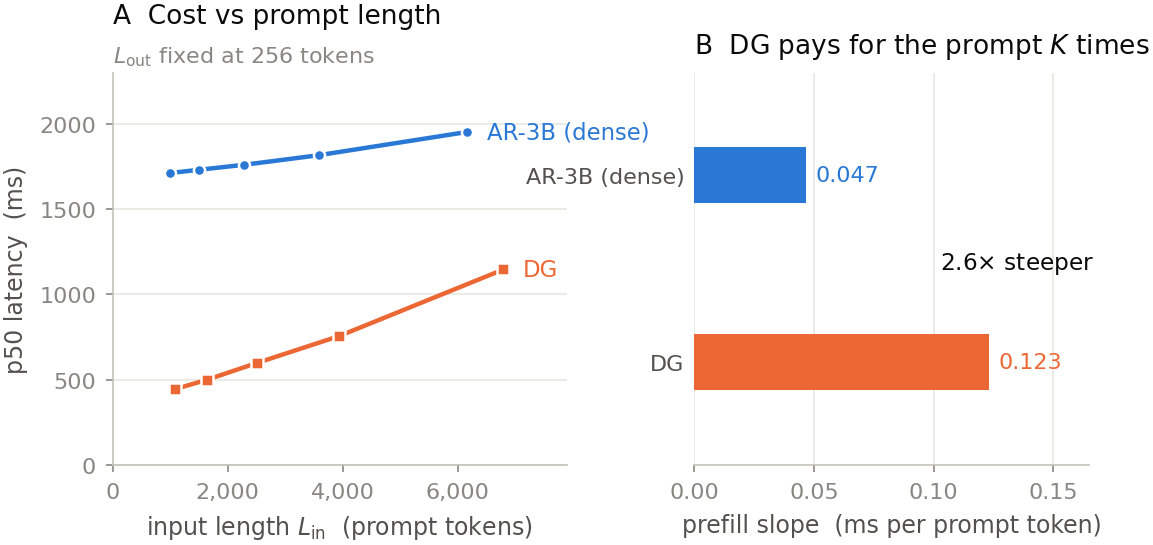
\includegraphics[width=\linewidth]{figures/fig3_input_sweep.png}
\caption{Input-length sweep at fixed $L_{\mathrm{out}}{=}\canvasLength$
(BGL, $n{=}100$; AR arm is dense AR-3B). The prompt is lengthened by
repeating the schema block, so the task is unchanged.}
\label{fig:input}
\end{figure}

\subsection{A free Pareto improvement at canvas $= 128$}

At canvas $=128$ the base falls to \canvasOneTwentyEightBase\,ms
($-2.0\%$) \emph{and} 9-field F1 rises to
\canvasOneTwentyEightFone{}, an improvement on both axes
simultaneously. At canvas $=64$ the base rises $48\%$ because the
per-canvas fixed overhead is paid twice as often; that setting is not
viable. Block size, not denoising schedule, is the interesting design
variable. Canvas $=128$ barely moves the crossover, $L^{*}$ falls
from $48$ to $46$ tokens, because the base drops only $2\%$, but
canvas $=64$ pushes it to $L^{*}\approx73$, since $L^{*}$ scales with
the base and that base is $48\%$ higher. Shrinking the canvas doesn't
shrink the prefill it must re-attend, so a smaller canvas buys
finer-grained output at the cost of paying the fixed overhead more
often.

\subsection{Joint canvas$\times$K sweep confirms canvas $= 128$ is
Pareto-optimal}

A full $4\times5$ grid (canvas $\in \{64,128,256,512\}$, $K \in
\{2,4,8,16,32\}$, $n{=}200$ per cell) confirms the single-knob finding
holds across all $K$ values, not just $K{=}8$. The Pareto frontier
contains six cells; the paper's current operating point (canvas$=256$,
$K{=}8$: p50$=$376\,ms, F1$=$0.853) is \emph{dominated} by
(canvas$=128$, $K{=}8$: p50$=$368\,ms, F1$=$0.864), which is faster
and higher quality simultaneously. The $K$ knee also shifts left at
smaller canvas: at canvas$=128$, $K{=}8$ is near saturation
(F1$=$0.864), while at canvas$=256$ quality keeps improving through
$K{=}32$ (F1$=$0.862). Canvas$=64$ remains non-viable even at $K{=}32$
(F1$=$0.834, below the canvas$=256$ $K{=}8$ baseline). Full data in
\texttt{results/issue114\_joint\_sweep.json}.

\section{Quality vs output length}
\label{app:quality}

DG degrades gracefully against a \emph{time} budget
and catastrophically against an \emph{output-length} budget. At
$L{=}128$ the AR model retains \arFOneTwentyEight{} F1 and
\arValidTwentyEight\% schema validity, while DG falls
to \dgFOneTwentyEight{} and \dgValidTwentyEight\%. Which budget an
application faces decides which architecture is safer;
Figure~\ref{fig:quality} traces both curves.

\begin{figure}[ht!]
\centering
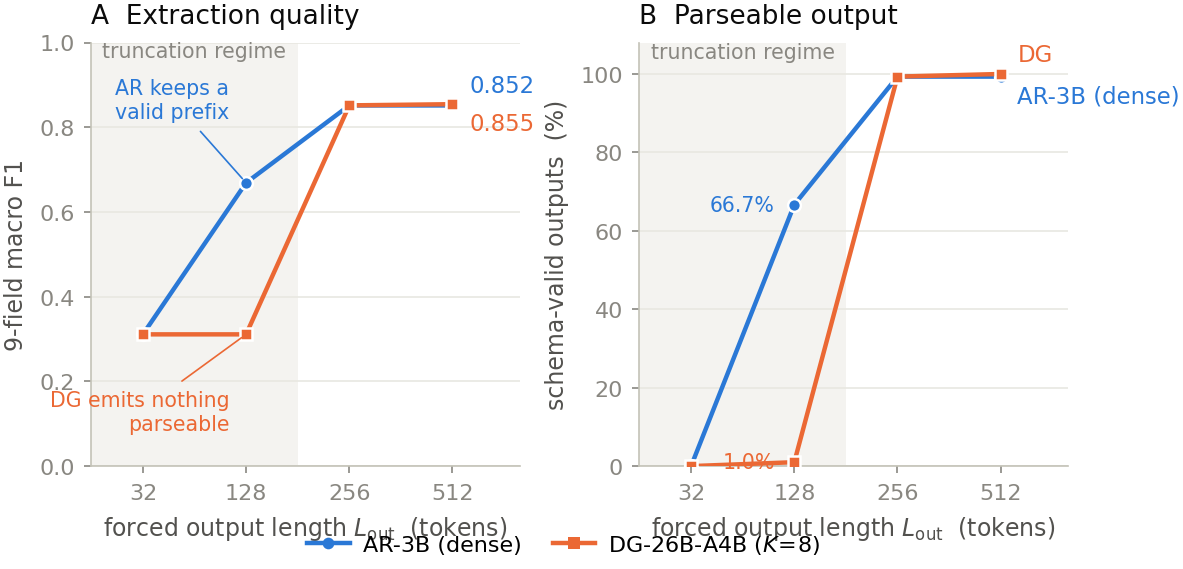
\includegraphics[width=\linewidth]{figures/fig5_quality_vs_length.png}
\caption{Quality and schema validity vs forced output length (BGL,
$n{=}300$; AR arm is dense AR-3B). \textbf{A:} DG's 9-field F1 rises
with $L$ and plateaus, while AR-3B is flat from $L{=}256$ to $L{=}512$
because first-object-wins parsing discards the rambled continuation.
\textbf{B:} schema validity is the sharper split, at $L{=}128$ DG
returns a valid record \dgValidTwentyEight\% of the time against
AR-3B's \arValidTwentyEight\%, because a canvas truncated below its
length is not a complete JSON object. This is the hard floor on DG's
completeness guarantee.}
\label{fig:quality}
\end{figure}

\section{Latency distributions}
\label{app:distributions}

The per-event latency distributions are asymmetric. Across 300 events at
$L{=}\canvasLength$:
\begin{itemize}[nosep]
\item AR-3B (dense baseline) per-event CV: \arEventCV\%; max/median: \arMaxMed$\times$.
\item DG-26B-A4B per-event CV: \dgEventCV\%; max/median: \dgMaxMed$\times$.
\end{itemize}
AR's \arEventCV\% CV means its p50 is a reliable planning number;
the DG arm's \dgEventCV\% means a p99 SLA lands in a very different
place than p50 would suggest.

\section{Does the advantage survive natural long output?}
\label{app:forced}

Table~\ref{tab:niche} lets AR-30B stop at its natural EOS near 126
tokens, so its long-output rows are a plateau instead of a
measurement of long output; neither arm is forced there. The question
this appendix answers is what happens when the \emph{task} makes the
output long. A multi-record extraction task, emit a JSON array of
$N$ structured records from $N$ consecutive log lines, produces
output of roughly $N \times 140$ tokens naturally, without forcing.
A record inside an array costs slightly more than the 126 tokens of a
bare record, for the enclosing punctuation and indentation.
Table~\ref{tab:forced} applies the fitted cost laws
(Eqs.~\ref{eq:ar}--\ref{eq:dg}):

\begin{table}[ht!]
\centering
\caption{What the cost laws predict when the task itself makes output
long. Row 1 is measured; rows 2--4 apply Eqs.~\ref{eq:ar}--\ref{eq:dg}
at the natural output length of an $N$-record extraction. The
advantage grows here, the opposite of
Table~\ref{tab:niche}. AR is no longer stopped by EOS at
126 tokens, so its line keeps climbing while DG adds one bounded
canvas at a time.}
\label{tab:forced}
\begin{tabular}{@{}lrrrr@{}}
\toprule
Task & $L_{\mathrm{out}}$ & AR-30B (ms) & DG (ms) & Ratio \\
\midrule
Single record (unforced) & 126 & 945 & 379 & DG $2.5\times$ \\
Multi-record $N{=}2$ & 280 & 2051 & 498 & DG $4.1\times$ \\
Multi-record $N{=}4$ & 560 & 4067 & 618 & DG $6.6\times$ \\
Multi-record $N{=}8$ & 1120 & 8099 & 857 & DG $9.5\times$ \\
\bottomrule
\end{tabular}
\end{table}

So the figure quoted in the abstract is the conservative
reading, not the optimistic one: it describes AR at its natural output
length. When the task genuinely demands a thousand tokens, the
staircase pulls further ahead, not less.

\section{Why the batching ceiling is likely architectural}
\label{app:batching_architectural}

Autoregressive batching is cheap because of KV-cache reuse: shared
prefixes are computed once, and each request's KV cache persists across
decode steps. Block-diffusion invalidates both forms of reuse:
\begin{enumerate}[nosep]
\item \textbf{Cross-request prefix sharing} requires that both requests
are at the same denoising step. Requests at different $K$ steps can't
share a KV cache because the attention mask differs per step.
\item \textbf{Within-request KV persistence} across denoising steps
fails because the denoising tokens' KV changes at every step (the mask
changes), so per-step computation can't reuse previous activations.
\end{enumerate}
Each denoising step is a fresh forward pass over the full sequence with
a different attention mask. The GPU does the same FLOPs whether batching
or not, different from AR decoding, where the attention
pattern is causal and the KV cache grows monotonically. A patched vLLM
might raise the DG multiplier to $\sim 2$--$3\times$, still an order of
magnitude below the dense AR-3B's $26$--$43\times$ and more than an
order below the AR-30B MoE's $25\times$.

\section{Cost-shape generalisation: code generation on HumanEval}
\label{app:humaneval}

The cost laws of \S\ref{sec:laws} are derived from structured log
extraction (BGL). Every experiment in the main text --- chains,
bounded deadline, wide schema, perturbation --- runs on the same task.
This appendix tests whether the line-vs-staircase cost shape
generalises to a second task: code generation on
HumanEval~\cite{humaneval} (164 problems, Python function completion).

Code generation has the properties that favour block-diffusion: output
is long (50--300 tokens), truncation is catastrophic
(\texttt{SyntaxError} = pass@1 = 0), schema validity is enforced by
Python syntax, and batch-1 is the natural mode (IDE autocomplete,
runtime codegen).

\subsection{Baseline: cost law holds on code}

Both arms were run serial (batch-1) on the pinned stack
(\S\ref{sec:threats}), $n{=}164$ problems.

\begin{table}[h]
\centering
\caption{HumanEval baseline (serial, batch-1, $n{=}164$). The cost-shape
law holds on code: AR scales linearly at 6.4\,ms/token (vs 7.2 on logs),
DG is a flat staircase. AR is 2.9$\times$ slower at natural output
(vs 2.5$\times$ on logs) --- the ratio is in the same range.}
\label{tab:humaneval}
\begin{tabular}{@{}lrrrrr@{}}
\toprule
Arm & pass@1 & code valid\% & p50 (ms) & mean tokens & ms/token \\
\midrule
DG K=8  & 0.287 & 31.1 & 280 & 99.5  & --- (staircase) \\
AR-30B  & 0.720 & 93.9 & 800 & 124.1 & 6.4 \\
AR-3B   & 0.573 & 99.4 & 560 & 107.7 & 5.2 \\
\bottomrule
\end{tabular}
\end{table}

AR-30B's per-token slope on code is close to its log-extraction slope.
DG's p50 is a single-canvas staircase cost, independent of output
length. The AR/DG ratio matches the log-extraction ratio --- the cost
shape generalises.

DG's lower pass@1 is expected: DiffusionGemma was trained as a
log-extraction model, not a code model. No code-trained block-diffusion
model exists at this scale; DiffusionGemma-26B-A4B is the only
open-weights block-diffusion model large enough for structured generation.
Instead, we evaluate
What matters is not absolute quality but whether the \emph{shape}
(line vs staircase) transfers.

\subsection{Deadline-bounded pass@1: AR collapses, DG stays flat}

Under a tightening deadline, AR's \texttt{max\_tokens} is set to
$\lfloor D / \text{slope} \rfloor$ (what it can generate in time).
DG always generates a full canvas regardless of $D$.

\begin{table}[h]
\centering
\caption{pass@1 under tightening deadline ($n{=}164$, serial). AR
collapses to 0.085 at $D{=}200$\,ms (truncated code = SyntaxError).
DG stays at 0.287 regardless of $D$ (always emits a complete canvas).
Crossover at $D \leq 400$\,ms: DG wins despite being worse at code.}
\label{tab:deadline}
\begin{tabular}{@{}rrrrrr@{}}
\toprule
$D$ (ms) & AR pass@1 & AR valid\% & AR p50 (ms) & DG pass@1 & DG p50 (ms) \\
\midrule
200  & 0.085 & 22.6 & 230 & 0.287 & 279 \\
400  & 0.189 & 33.5 & 434 & 0.287 & 280 \\
600  & 0.274 & 45.7 & 637 & 0.287 & 280 \\
800  & 0.311 & 54.3 & 801 & 0.287 & 280 \\
$\infty$ & 0.720 & 93.9 & 800 & 0.287 & 280 \\
\bottomrule
\end{tabular}
\end{table}

AR collapses because a truncated function is a \texttt{SyntaxError},
not just a lower-quality answer. On logs, truncation means missing
JSON keys (bad but recoverable); on code, it means a crash. This makes
the graceful-degradation property (drop $K$, keep completeness)
visibly more valuable on code than on logs.

\subsection{Multi-turn correction chain: per-hop latency stays flat}

A code correction chain tests whether DG's per-hop latency stays
constant across \emph{variable-content} rounds (generate $\to$ execute
$\to$ fix $\to$ re-execute), not just repeated identical calls. Up to
5 rounds per problem.

\begin{table}[h]
\centering
\caption{Multi-turn correction chain ($n{=}164$, serial, max 5 rounds).
DG's per-round latency stays flat ($+6\%$); AR's grows ($+21\%$) as
fix prompts accumulate context. Both saturate by round 3.}
\label{tab:chain}
\begin{tabular}{@{}lrrrr@{}}
\toprule
Arm & R1 pass@1 & cumulative & R1 p50 (ms) & total p50 (ms) \\
\midrule
DG K=8  & 0.854 & 0.957 & 287 & 305 \\
AR-30B  & 0.762 & 0.896 & 511 & 620 \\
\bottomrule
\end{tabular}
\end{table}

DG's total p50 (305\,ms) is barely above its single-round p50
(287\,ms), because most problems solve in round 1 and the few that
need a fix round add little. AR's total (620\,ms) is $1.2\times$ its
single-round latency (511\,ms), because the fix round re-prefills a
longer accumulated prompt. The staircase shape holds across
variable-content hops, confirming the chain latency claim from
\S\ref{sec:survives} with a real multi-turn workflow.


% NeurIPS Paper Checklist (placed after references/appendices, page-limit-exempt)
\section*{NeurIPS Paper Checklist}
\label{app:neurips_checklist}

\begin{enumerate}[leftmargin=2em,label=\arabic*.,itemsep=4pt]

\item \textbf{Claims.}
\emph{Yes.} The abstract and introduction state the cost-shape
comparison, the crossover length, and the five conditions. Every claim
is grounded in measured data; the scope is explicitly limited to the
BGL/HDFS log-extraction task and the two matched models
(\S\ref{sec:intro}, \S\ref{sec:threats}).

\item \textbf{Limitations.}
\emph{Yes.} \S\ref{sec:threats} discusses all threats to validity:
single-GPU measurement, single-dataset scope (BGL), the quality/latency
arm mismatch, grammar-constrained AR not tested, and the engine-bounded
batching ceiling.

\item \textbf{Theory, Assumptions and Proofs.}
\emph{Yes.} The cost laws (Eqs.~\ref{eq:ar}--\ref{eq:lcross}) are
fitted from measurement with stated $R^2$ values; the crossover
derivation is given in full (\S\ref{sec:laws}).

\item \textbf{Experimental Result Reproducibility.}
\emph{Yes.} All code, result artifacts, and provenance blocks are in
the project repository. \texttt{AGENTS.md} documents exact commands;
\texttt{verify\_numbers.py} asserts that macros match artifacts
(\S\ref{sec:threats}, Reproducibility paragraph).

\item \textbf{Open Access to Data and Code.}
\emph{Yes.} BGL and HDFS are from LOGHUB (MIT licence). All measurement
scripts are in \texttt{models/experiments/}. The pinned stack is
vLLM 0.25.1 / torch 2.11.0 / CUDA 13.0.

\item \textbf{Experimental Setting/Details.}
\emph{Yes.} Data splits (\S\ref{sec:intro}), hyperparameters
(temperature$=$0, $K{=}8$, canvas$=$256), and model configurations are
stated in \S\ref{sec:intro} and each result artifact's
\texttt{provenance} block.

\item \textbf{Experiment Statistical Significance.}
\emph{Yes.} Bootstrap 95\% CIs are reported for both arms (AR-30B
[918, 927]\,ms, DG [379, 380]\,ms). A permutation test on the
difference of medians gives $p < 10^{-5}$. Seed-to-seed CV is
$0.04\%$ across 3 seeds (\S\ref{sec:wins}, \S\ref{sec:threats}).

\item \textbf{Experiments Compute Resources.}
\emph{Yes.} Single A100 80GB GPU. Total $\sim$20 GPU-hours for
reported experiments; $\sim$10 additional for preliminary/failed runs.
Serial cell takes $\sim$2 min; per-event timings are reported
(\S\ref{sec:threats} footnote).

\item \textbf{Code of Ethics.}
\emph{Yes.} This work conforms to the NeurIPS Code of Ethics. It is an
efficiency analysis of existing public models on public data; no new
model is released and no human subjects are involved
(\S\ref{sec:threats}, Ethics paragraph).

\item \textbf{Broader Impacts.}
\emph{Yes.} The paper identifies a latency regime where block-diffusion
decoding is faster than autoregressive decoding. The positive impact is
reduced inference cost for serial, latency-sensitive deployments
(security operations, autonomous driving). The negative impact is that
cheaper inference could accelerate LLM deployment in high-stakes
settings where errors are costly; the paper's explicit scope-limiting
(five conditions) and its disclosure of where diffusion fails
(\S\ref{sec:survives}) are the mitigations within the paper's scope.

\item \textbf{Safeguards.}
\emph{N/A.} No new model is released. The paper analyses existing
publicly available models (DiffusionGemma, Qwen3) on public log data.

\item \textbf{Licences.}
\emph{Yes.} BGL/HDFS: LOGHUB, MIT. Drain: \texttt{drain3}, Apache 2.0.
vLLM: Apache 2.0. DiffusionGemma: Gemma Terms of Use. Qwen3:
Apache 2.0. LLaDA-8B-Instruct: MIT (\S\ref{sec:threats} footnote).

\item \textbf{New Assets.}
\emph{N/A.} No new datasets, models, or code packages are released.

\item \textbf{Crowdsourcing and Research with Human Subjects.}
\emph{N/A.} No crowdsourcing or human-subjects research was conducted.

\item \textbf{IRB Approvals.}
\emph{N/A.} No human-subjects research; no IRB review required.

\item \textbf{Declaration of LLM Usage.}
\emph{Yes.} The core method involves running LLMs (DiffusionGemma-26B,
Qwen3-30B-A3B) as the systems under test. LLMs are the subject of the
analysis, not a tool used in the research methodology. No LLM was used
for writing or editing.

\end{enumerate}


\end{document}
